%%%%%%%%%%%%%%%%%%%%%%%%%%%%%%%%%%%%%%%%% 
% WAGASCI Hardware and Software Documentation
% Version 0.1 (7/11/2018)
% 
% License:
% CC BY-NC-SA 3.0 (http://creativecommons.org/licenses/by-nc-sa/3.0/)
% 
% Created by:
% Pintaudi Giorgio, Yokohama National University
% giorgio-pintaudi-kx@ynu.jp

%%%%%%%%%%%%%%%%%%%%%%%%%%%%%%%%%%%%%%%%% 

% -------------------------------LATEX SYNTAX----------------------------------
% 
% enter:               \\, \linebreak, \newline
% new page:            \newpage
% new section:         \section{name} text
% new paragraph        \subsection{name} text  (subsub...section{name} for more layers)
%       % , &, $, _, etc:     (these are latex operators, add a "\" to type it as text)
% add comment:         \commred{text}, \commblue{text}, \commpurp{text}, \commgreen{text}
% clean code:          \cleancode{text}
% idem without indent: \cleanstyle{text}
% bold, italic, under: \textbf{text}, textit{text}, \underline{text}
% table:               \begin{tabular}{c c c} text \end{tabular}
% ('&' for tab, '\\' for new 
% 
% ------------------------------------------------------------------------------
% chktex-file 1
% chktex-file 13
% chktex-file 29
% chktex-file 44

\documentclass[a4paper]{report}

\usepackage[utf8]{inputenc}
\usepackage[T1]{fontenc}
\usepackage{CJKutf8}
\usepackage{epigraph}
\usepackage{amsmath}
\usepackage{colortbl}
\usepackage{xcolor}
\usepackage{array}
\usepackage{xtab}
\usepackage{booktabs}
\usepackage{pbox}
\usepackage{graphicx}
\usepackage{subcaption}
\usepackage{grffile}
\usepackage{fancyref}
\usepackage{hyperref}
\usepackage{float}
\usepackage{scrextend}
\usepackage{setspace}
\usepackage{xargs}
\usepackage{multicol}
\usepackage{nameref}
\usepackage{sectsty}
\usepackage{enumitem}
\usepackage{geometry}
\usepackage{listings}
\usepackage[export]{adjustbox}
\usepackage{textcomp}
\usepackage[backend=biber]{biblatex}

% bibliography file
\addbibresource{./bibliography.bib}

% page format
% \geometry{
%   a4paper,
%   total={170mm,257mm},
%   left=20mm,
%   top=20mm,
% }

% add padding to tables
\renewcommand{\arraystretch}{1.5}

% images folder location
\graphicspath{ {images/} }

% blue links
\hypersetup{colorlinks=true, linkcolor=blue}

% Keep all footnotes on the according page
\interfootnotelinepenalty=10000

% \subsubsectionfont{\large}
% \subsectionfont{\Large}
% \sectionfont{\LARGE}

% define various colors
\definecolor{dkgreen}{rgb}{0,0.6,0}
\definecolor{gray}{rgb}{0.5,0.5,0.5}
\definecolor{mauve}{rgb}{0.58,0,0.82}
\definecolor{cleanOrange}{HTML}{D14D00}
\definecolor{cleanYellow}{HTML}{FFFF99}
\definecolor{cleanBlue}{HTML}{3d0099}
\colorlet{Red}{red}
\colorlet{Blue}{blue}
\colorlet{Green}{green}
\colorlet{Purple}{purple}
\newcommand{\cleanstyle}[1]{\text{\textcolor{cleanOrange}{\texttt{#1}}}}

% formatting for bash language
\lstset{frame=tb,
  language=bash,
  aboveskip=3mm,
  belowskip=3mm,
  showstringspaces=false,
  columns=flexible,
  basicstyle={\small\ttfamily},
  numbers=none,
  numberstyle=\tiny\color{gray},
  keywordstyle=\color{blue},
  commentstyle=\color{dkgreen},
  stringstyle=\color{mauve},
  breaklines=true,
  breakatwhitespace=true,
  tabsize=3
}
\makeatletter
\providecommand*{\toclevel@lstlisting}{0}
\makeatother

% add colored comments
\usepackage[colorinlistoftodos,prependcaption,textsize=footnotesize]{todonotes}
\newcommandx{\commred}[2][1=]{\textcolor{Red}
  {\todo[linecolor=red,backgroundcolor=red!25,bordercolor=red,#1]{#2}}}
\newcommandx{\commblue}[2][1=]{\textcolor{Blue}
  {\todo[linecolor=blue,backgroundcolor=blue!25,bordercolor=blue,#1]{#2}}}
\newcommandx{\commgreen}[2][1=]{\textcolor{OliveGreen}{\todo[linecolor=OliveGreen,
    backgroundcolor=OliveGreen!25,bordercolor=OliveGreen,#1]{#2}}}
\newcommandx{\commpurp}[2][1=]{\textcolor{Plum}{\todo[linecolor=Plum,
    backgroundcolor=Plum!25,bordercolor=Plum,#1]{#2}}}

% ------------------------------------BEGIN DOC---------------------------------------

\begin{document}
% \selectlanguage{english}

\title{WAGASCI ELECTRONICS\\USER GUIDE}
\author{\\Author: Pintaudi Giorgio\\\\
  Physics Department, Yokohama National University\\
  240-8501 Yokohama-shi Hodogaya-ku Tokiwadai 79-5\\ % chktex-file 8
  Minamino Laboratory\\
  Email: giorgio-pintaudi-kx@ynu.jp\\
  Phone: (+81) 070-4122-3907\\} \date{\today}
\maketitle
\newpage

% -----------------------------------------TOC---------------------------------------
\tableofcontents\label{c}
\newpage

% ------------------------------------------TEXT-------------------------------------

\chapter{WAGASCI electronics}
In this chapter the DAQ electronics of the WAGASCI experiment is described in as
much detail as possible. With this statement, I don't mean that I am going to
write down again everything that there is to know about the WAGASCI electronics:
if there is any source that contains some relevant piece of information, I am
going to cite that reference and consider that content as covered.

\section{Overview}\label{sec:overview}
The WAGASCI DAQ system electronics is composed of many different boards
(Figure~\ref{DAQ-schematics}). All of them were developed at LLR (Laboratoire
Leprince-Ringuet) in France. Please refer to the following articles for an
introduction to every board of the
system\cite{Gastaldi:2014vaa,Gastaldi:2014oid}.  Be warned that these articles
and all the ones that follow through the chapter, describe the general features
of the DAQ system but don't explain how to actually use it. Moreover they are
somewhat redundant, so if you choose to read them all, be prepared to read the
same things over and over again. I cannot blame the authors too much for this
kind of ``publication'' spamming. If I were them, after so much effort to
develop a new DAQ system (both hardware and software), I would like at least to
get as many publications as possible out of it, too.

On the other hand this very documentation is meant more as a ``User Guide'', so,
while referring to the said literature for the more general and technical
remarks, I will only focus on practical usage scenarios and examples.
\begin{figure}[H]
  \centering \includegraphics[width=0.7\linewidth]{DAQ-schematics-1} \\
  \includegraphics[width=0.7\linewidth]{DAQ-schematics-2}
  \caption{Schematics of the WAGASCI DAQ system electronics. These figure only
    shows the connections for a single DIF. The maximum theoretical number of
    ASUs for a single DIF is 4x256 but no more than 4x5 is needed for
    WAGASCI.}\label{DAQ-schematics}
\end{figure}
\begin{figure}[H]
  \centering
  \begin{minipage}{0.48\linewidth}
    \centering
    \includegraphics[width=0.8\linewidth]{WAGASCI-open-view} \\
    \includegraphics[width=0.98\linewidth]{DAQ-overview-WAGASCI}
    \caption{\small Schematics of WAGASCI boards and connections for a single
      detector. For two detectors everything doubles but the GDCC, CCC and DAQ
      PC}\label{fig:DAQ-overview-WAGASCI}
  \end{minipage}%
  \begin{minipage}{0.48\linewidth}
    \centering
    \includegraphics[width=0.8\linewidth]{SideMRD-open-view} \\
    \includegraphics[width=0.98\linewidth]{DAQ-overview-SideMRD}
    \caption{\small Schematics of SideMRD boards and connections for a single
      detector. For two detectors everything doubles but the GDCC, CCC and DAQ
      PC}\label{fig:DAQ-overview-SideMRD}
  \end{minipage}
\end{figure}

\subsection{List of boards, connectors and cables}
In this section, I try to list some of the boards, connectors and cables for the
WAGASCI experiment. I only focus on the parts that we may need to (re)-purchase
in future. This is not meant to be a thorough list but more like a memo to my future
self if we ever have to shop for spares or replacements.

\begin{figure}[H]
    \centering
    \includegraphics[width=0.7\linewidth,frame]{WAGASCI-housing-schematics}
    \caption{Schematics of the WAGASCI housing
      connectors}\label{fig:WAGASCI-housing-schematics}
  \end{figure}
\commred{To check if the connectors really match with the figure}
  
{{
\definecolor{latextbl}{RGB}{78,130,190}
\setlength{\extrarowheight}{1pt}
\setlength\arrayrulewidth{1pt}\setlength\doublerulesep{0pt}
\arrayrulecolor{white}\doublerulesepcolor{black}
\bottomcaption[Housing feedthrough connectors]{Housing feedthrough connectors. }
\label{table:housing}

\tablehead{\hline
\rowcolor{latextbl}\multicolumn{1}{|>{\columncolor{latextbl}}c|}{\color{white}\textbf{Feedthrough connector}} & \multicolumn{1}{>{\columncolor{latextbl}}c|}{\color{white}\textbf{\#}} & \multicolumn{1}{>{\columncolor{latextbl}}c|}{\color{white}\textbf{Remarks}} & \multicolumn{1}{>{\columncolor{latextbl}}c|}{\color{white}\textbf{Reference}} \\
\hline
\hline
}
\tabletail{\hline
\hline
\multicolumn{4}{|r|}{{Continued on next page}} \\
\hline
}
\tablelasttail{}
\begin{center}
\begin{xtabular}{|l|c|l|l|}
\rowcolor{latextbl!25}HDMI                    & 2 & GDCC-IF                       & \href{https://jp.rs-online.com/web/p/hdmi-connectors/9093717/}{RS 909-3717}                      \\
\hline
\rowcolor{latextbl!10}SHV (Safe High Voltage) & 2 & HV-IF                         & \href{https://jp.rs-online.com/web/p/shv-connectors/2127444/}{RS 212-7444}                       \\
\hline
\rowcolor{latextbl!25}Binder 5 contacts       & 2 & LV-IF                         & \href{https://www.binder-connector.de/pdfsheets/download/en/09+0115+80+05}{Binder 09-0115-80-05} \\
\hline
\rowcolor{latextbl!10}Binder 6 contacts       & 2 & JTAG for DIF firmware upgrade & \href{http://www.binder-connector.com/pdfsheets/download/en/09+0123+80+06}{Binder 09-0123-80-06} \\
\hline
\rowcolor{latextbl!25}Binder 14 contacts      & 2 & For DIF LED                   & \href{https://www.binder-connector.de/pdfsheets/download/en/09+0453+80+14}{Binder 09-0453-80-14} \\
\hline
\end{xtabular}
\end{center}
} 
\commblue{Binder connectors are currently not on sale in
    Japan. They may appear again on sale on RS Japan in future.}}

{{
\definecolor{latextbl}{RGB}{78,130,190}
\setlength{\extrarowheight}{1pt}
\setlength\arrayrulewidth{1pt}\setlength\doublerulesep{0pt}
\arrayrulecolor{white}\doublerulesepcolor{black}
\bottomcaption[Cables and connectors for inside the housing]{Cables and connectors for inside the housing. }
\label{table:cables-internal}

\tablehead{\hline
\rowcolor{latextbl}\multicolumn{1}{|>{\columncolor{latextbl}}c|}{\color{white}\textbf{Purpose}} & \multicolumn{1}{>{\columncolor{latextbl}}c|}{\color{white}\textbf{Cables/Connectors}} & \multicolumn{1}{>{\columncolor{latextbl}}c|}{\color{white}\textbf{\#}} & \multicolumn{1}{>{\columncolor{latextbl}}c|}{\color{white}\textbf{Remarks}} & \multicolumn{1}{>{\columncolor{latextbl}}c|}{\color{white}\textbf{Reference}} \\
\hline
\hline
}
\tabletail{\hline
\hline
\multicolumn{5}{|r|}{{Continued on next page}} \\
\hline
}
\tablelasttail{}
\begin{center}
\begin{xtabular}{|l|l|l|l|l|}
\rowcolor{latextbl!25}\textbf{DIF data}  & 50cm HDMI              & 2  & to DIF    & Any cable is good                                                                                                     \\
\hline
\rowcolor{latextbl!10}\textbf{IF LV}     & 50cm LV wire           & 2  & to IF LV  & \href{https://www.digikey.jp/product-detail/ja/alpha-wire/6305-SL005/A6305SL-100-ND/3714712}{Digi-Key A6305SL-100-ND} \\
\hline
\rowcolor{latextbl!25}                   & MOLEX contacts         & 10 & to IF LV  & \href{https://jp.rs-online.com/web/p/pcb-connector-contacts/6706445}{RS 670-6445}                                     \\
\hline
\rowcolor{latextbl!10}                   & MOLEX housing          & 2  & to IF LV  & \href{https://jp.rs-online.com/web/p/pcb-connector-housings/6704174}{RS 670-4174}                                     \\
\hline
\rowcolor{latextbl!25}\textbf{DIF flash} & JTAG housing           & 2  & to DIF    & \href{https://jp.rs-online.com/web/p/pcb-connector-housings/6737626/}{RS 673-7626}                                    \\
\hline
\rowcolor{latextbl!10}                   & JTAG contacts          & 20 & to DIF    & \href{https://jp.rs-online.com/web/p/pcb-connector-contacts/7142404/}{RS 714-2404}                                    \\
\hline
\rowcolor{latextbl!25}\textbf{LED}       & 15 wires cable         & 2  & Extra LED & \href{https://www.digikey.jp/products/ja?keywords=ALPHA%20WIRE%20%203470/15C%20SL005}{3470/15C SL005}                 \\
\hline
\rowcolor{latextbl!10}                   & ISDF  housing          & 2  & Extra LED & \href{https://jp.rs-online.com/web/p/pcb-connector-housings/1800450/}{RS 180-0450}                                    \\
\hline
\rowcolor{latextbl!25}                   & ISDF contacts          & 28 & Extra LED & \href{https://jp.rs-online.com/web/p/pcb-connector-contacts/1801564/}{RS 180-1564}                                    \\
\hline
\rowcolor{latextbl!10}\textbf{ASU}       & 10cm 50-pin flat cable & 64 & ASU-ASU   & \href{https://jp.rs-online.com/web/p/serial-cable-assemblies/9011848/}{RS 901-1848}                                   \\
\hline
\rowcolor{latextbl!25}                   & 22cm 50-pin flat cable & 16 & ASU-IF    & \href{https://jp.rs-online.com/web/p/serial-cable-assemblies/9011857/}{RS 901-1857}                                   \\
\hline
\rowcolor{latextbl!10}\textbf{HV}        & LEMO                   & 2  & to IF HV  & \href{https://jp.rs-online.com/web/p/industrial-automation-circular-connectors/3202568}{RS 320-2568}                  \\
\hline
\end{xtabular}
\end{center}
} 
\commred{To check where the LED cable have to be
    connected}}

{{
\definecolor{latextbl}{RGB}{78,130,190}
\setlength{\extrarowheight}{1pt}
\setlength\arrayrulewidth{1pt}\setlength\doublerulesep{0pt}
\arrayrulecolor{white}\doublerulesepcolor{black}
\bottomcaption[Cables and connectors for outside the housing]{Cables and connectors for outside the housing. }
\label{table:cables-external}

\tablehead{\hline
\rowcolor{latextbl}\multicolumn{1}{|>{\columncolor{latextbl}}c|}{\color{white}\textbf{Purpose}} & \multicolumn{1}{>{\columncolor{latextbl}}c|}{\color{white}\textbf{Cables/Connectors}} & \multicolumn{1}{>{\columncolor{latextbl}}c|}{\color{white}\textbf{\#}} & \multicolumn{1}{>{\columncolor{latextbl}}c|}{\color{white}\textbf{Remarks}} & \multicolumn{1}{>{\columncolor{latextbl}}c|}{\color{white}\textbf{Reference}} \\
\hline
\hline
}
\tabletail{\hline
\hline
\multicolumn{5}{|r|}{{Continued on next page}} \\
\hline
}
\tablelasttail{}
\begin{center}
\begin{xtabular}{|l|l|l|l|l|}
\rowcolor{latextbl!25}\textbf{DIF data}     & ?cm HDMI                  & 2 & to GDCC     & Any cable is good                                                                                                           \\
\hline
\rowcolor{latextbl!10}\textbf{IF LV}        & Binder 5 contacts (plug)  & 2 & to LV       & \href{https://www.binder-connector.de/pdfsheets/download/en/99+5114+00+05}{Binder 99-5114-00-05}                            \\
\hline
\rowcolor{latextbl!25}                      & Crimping terminals        & 4 & to LV PSU   & \href{https://jp.rs-online.com/web/p/crimp-ring-terminals/6048389/}{RS 604-8389}                                            \\
\hline
\rowcolor{latextbl!10}\textbf{DIF firmware} & Binder 6 contacts (plug)  & 2 & to DIF      & \href{https://www.binder-connector.de/pdfsheets/download/en/99+5122+00+06}{Binder 99-5122-00-06}                            \\
\hline
\rowcolor{latextbl!25}                      & JTAG cable's wires        & 2 & to XILINX   & \href{https://lappjapan.lappgroup.com/fileadmin/documents/technische_doku/datenblaetter/unitronic/DB0034302EN.pdf}{0034302} \\
\hline
\rowcolor{latextbl!10}\textbf{LED}          & Binder 14 contacts (plug) & 2 & to LED      & \href{https://www.binder-connector.de/pdfsheets/download/en/99+5452+00+14}{Binder 99-5452-00-14}                            \\
\hline
\rowcolor{latextbl!25}\textbf{IF HV}        & SHV connector female      & 2 & to HV       & \href{https://jp.rs-online.com/web/p/shv-connectors/2127438/}{RS 212-7438}                                                  \\
\hline
\rowcolor{latextbl!10}                      & BNC 50$\Omega$            & 2 & to HV PSU   & \href{https://jp.rs-online.com/web/p/bnc-connectors/5464853}{RS 546-4853}                                                   \\
\hline
\rowcolor{latextbl!25}                      & Coaxial Cable             & 2 & 50 $\Omega$ & \href{https://jp.rs-online.com/web/p/coaxial-cable/2228610/}{RS 222-8610}                                                   \\
\hline
\rowcolor{latextbl!10}                      & DSUB connector            & 2 & to HV PSU   & ???                                                                                                                         \\
\hline
\end{xtabular}
\end{center}
} 
\commred{To check the length of the HDMI cables and the
    model of the DSUB cable}}

{{
\definecolor{latextbl}{RGB}{78,130,190}
\setlength{\extrarowheight}{1pt}
\setlength\arrayrulewidth{1pt}\setlength\doublerulesep{0pt}
\arrayrulecolor{white}\doublerulesepcolor{black}
\bottomcaption[Cables for beam trigger and spill number processing]{Cables for beam trigger and spill number processing. }
\label{table:cables-beam-trigger}

\tablehead{\hline
\rowcolor{latextbl}\multicolumn{1}{|>{\columncolor{latextbl}}c|}{\color{white}\textbf{Cables/Connectors}} & \multicolumn{1}{>{\columncolor{latextbl}}c|}{\color{white}\textbf{\#}} & \multicolumn{1}{>{\columncolor{latextbl}}c|}{\color{white}\textbf{Remarks}} & \multicolumn{1}{>{\columncolor{latextbl}}c|}{\color{white}\textbf{Reference}} \\
\hline
\hline
}
\tabletail{\hline
\hline
\multicolumn{4}{|r|}{{Continued on next page}} \\
\hline
}
\tablelasttail{}
\begin{center}
\begin{xtabular}{|l|c|l|l|}
\rowcolor{latextbl!25}Flat cable (34 wires)         & 1 & spill number (ECL signal)      & ???                                                                     \\
\hline
\rowcolor{latextbl!10}Hirose connector (10 pins)    & 2 & TTL input (on ZedBoard)        & \href{https://jp.rs-online.com/web/p/pcb-headers/8960809/}{RS 896-0809} \\
\hline
\rowcolor{latextbl!25}8ch. LEMO - 10-pin flat cable & 2 & TTL signal (to Pmod connector) & ???                                                                     \\
\hline
\end{xtabular}
\end{center}
} 
\commred{To check the references}}

{{
\definecolor{latextbl}{RGB}{78,130,190}
\setlength{\extrarowheight}{1pt}
\setlength\arrayrulewidth{1pt}\setlength\doublerulesep{0pt}
\arrayrulecolor{white}\doublerulesepcolor{black}
\bottomcaption[Items on the WAGASCI rack]{Items on the WAGASCI rack. }
\label{table:rack}

\tablehead{\hline
\rowcolor{latextbl}\multicolumn{1}{|>{\columncolor{latextbl}}c|}{\color{white}\textbf{Item}} & \multicolumn{1}{>{\columncolor{latextbl}}c|}{\color{white}\textbf{Remarks}} & \multicolumn{1}{>{\columncolor{latextbl}}c|}{\color{white}\textbf{Reference}} \\
\hline
\hline
}
\tabletail{\hline
\hline
\multicolumn{3}{|r|}{{Continued on next page}} \\
\hline
}
\tablelasttail{}
\begin{center}
\begin{xtabular}{|l|l|l|}
\rowcolor{latextbl!25}Switch (Hub)             & NETGEAR 16 Port Switch                                                         & \href{https://www.netgear.com/support/product/jgs516.aspx}{JGS512 v2}                                         \\
\hline
\rowcolor{latextbl!10}NIM crate                & Large current type                                                             & \href{https://www.h-repic.co.jp/products/module/crates_nim/rpn_005_153}{RPN-005-153}                          \\
\hline
\rowcolor{latextbl!25}VME crate                & \pbox{4cm}{special processing RPPV-2016W (without J2, rail positions changed)} & ???                                                                                                           \\
\hline
\rowcolor{latextbl!10}Front-end DAQ PC         & DAQ PC                                                                         & \href{https://www.dell.com/en-us/work/shop/productdetailstxn/poweredge-r330}{Dell PowerEdge R330 Rack Server} \\
\hline
\rowcolor{latextbl!25}Back-end Slow Control PC & ANA PC                                                                         & \href{https://www.dell.com/en-us/work/shop/povw/poweredge-r530}{Dell PowerEdge R530 Rack Server}              \\
\hline
\end{xtabular}
\end{center}
} 
\commred{To check the VME crate remarks meaning}}

{
\definecolor{latextbl}{RGB}{78,130,190}
\setlength{\extrarowheight}{1pt}
\setlength\arrayrulewidth{1pt}\setlength\doublerulesep{0pt}
\arrayrulecolor{white}\doublerulesepcolor{black}
\bottomcaption[Slow Control Items]{Slow Control Items. }
\label{table:slow-control}

\tablehead{\hline
\rowcolor{latextbl}\multicolumn{1}{|>{\columncolor{latextbl}}c|}{\color{white}\textbf{Item}} & \multicolumn{1}{>{\columncolor{latextbl}}c|}{\color{white}\textbf{Remarks}} & \multicolumn{1}{>{\columncolor{latextbl}}c|}{\color{white}\textbf{Reference}} \\
\hline
\hline
}
\tabletail{\hline
\hline
\multicolumn{3}{|r|}{{Continued on next page}} \\
\hline
}
\tablelasttail{}
\begin{center}
\begin{xtabular}{|l|l|l|}
\rowcolor{latextbl!25}PicoLog 1012      & Water Level sensor probe & \href{https://www.picotech.com/data-logger/picolog-1000-series/multi-channel-daq}{PicoLog 1012}            \\
\hline
\rowcolor{latextbl!10}TDK 200W 80V 2.5A & HV PSU                   & \href{https://product.tdk.com/en/search/power/switching-power/prg-power/info?part_no=ZUP80-2.5}{ZUP80-2.5} \\
\hline
\rowcolor{latextbl!25}TDK 200W 6V 33A   & LV PSU                   & \href{https://product.tdk.com/ja/search/power/switching-power/prg-power/info?part_no=ZUP6-33}{ZUP6-33}     \\
\hline
\end{xtabular}
\end{center}
} 


{
\definecolor{latextbl}{RGB}{78,130,190}
\setlength{\extrarowheight}{1pt}
\setlength\arrayrulewidth{1pt}\setlength\doublerulesep{0pt}
\arrayrulecolor{white}\doublerulesepcolor{black}
\bottomcaption[Cables and connectors for the DIF firware update]{Cables and connectors for the DIF firware update. }
\label{table:dif-firmware}

\tablehead{\hline
\rowcolor{latextbl}\multicolumn{1}{|>{\columncolor{latextbl}}c|}{\color{white}\textbf{Item}} & \multicolumn{1}{>{\columncolor{latextbl}}c|}{\color{white}\textbf{\#}} & \multicolumn{1}{>{\columncolor{latextbl}}c|}{\color{white}\textbf{Remarks}} & \multicolumn{1}{>{\columncolor{latextbl}}c|}{\color{white}\textbf{Reference}} \\
\hline
\hline
}
\tabletail{\hline
\hline
\multicolumn{4}{|r|}{{Continued on next page}} \\
\hline
}
\tablelasttail{}
\begin{center}
\begin{xtabular}{|l|c|l|l|}
\rowcolor{latextbl!25}DIF connector (housing)  & 2  & 8-contacts                    & \href{https://jp.rs-online.com/web/p/pcb-connector-housings/6737626/}{RS 673-7626}               \\
\hline
\rowcolor{latextbl!10}DIF connector (contacts) & 16 &                               & \href{https://jp.rs-online.com/web/p/pcb-connector-contacts/7142404/?sra=pstk}{RS 714-2404}      \\
\hline
\rowcolor{latextbl!25}Xilinx USB cable         & 1  & HW-USB-FLYLEADS-G             & \href{https://jp.rs-online.com/web/p/programmable-logic-development-kits/6973456/}{RS 697-3456 } \\
\hline
\rowcolor{latextbl!10}Binder 6 contacts        & 2  & JTAG for DIF firmware upgrade & \href{http://www.binder-connector.com/pdfsheets/download/en/09+0123+80+06}{Binder 09-0123-80-06} \\
\hline
\rowcolor{latextbl!25}Binder 6 contacts (plug) & 1  & to DIF                        & \href{https://www.binder-connector.de/pdfsheets/download/en/99+5122+00+06}{Binder 99-5122-00-06} \\
\hline
\end{xtabular}
\end{center}
} 


\arrayrulecolor{black}\doublerulesepcolor{black}

\subsection{References}
The documentation about the WAGASCI electronics is relatively vast but randomly
dispersed through the net. Here I am providing a compilation of all the
available literature that I could find.

\begin{itemize}
\item Master Theses about the WAGASCI electronics and DAQ system: Chikuma
  Naruhiro~\cite{Chikuma:2016}, Tamura Riku~\cite{Tamura:2018}.
\item Articles about the WAGASCI electronics (but not directly referring to the
  WAGASCI experiment):~\cite{Gastaldi:2014vaa,Gastaldi:2014oid,GDCC:2012}.
\item General articles about pre-amplifiers and amplifiers used for Physics
  measurements~\cite{Hamamatsu:2001,Bertuccio:1996,Lioliou:2015,Ortec} and
  everything about signal processing that you can find in the Knoll
  book~\cite{Knoll:2010radiation}. This should be enough to get you started. Of
  course there is much more online about Physical applications of pre-amplifier
  and amplifiers.  
\item Articles and slide shows about the SPIROC
  characterization~\cite{Callier:2008,Callier:2009,Fabbri:2009,%
    Callier:2013,Callier:2015}.
\item SPIROC manuals and
  pin-out~\cite{SPIROC2Dpinlist,SPIROC2Ddatasheet,SPIROC:OMEGA}.
\end{itemize}

\section{MPPC}
This section is only a stub. It is only meant as a list of calibration
parameters.

\subsection{Gain Calibration}
All gains are required to stay within 10\%.\commred{To write about calibration procedure}

\subsection{Arrayed MPPC}
\begin{itemize}
\item (SPIROC2D) PreAMP gain parameter = 49-50 (Fixed for each channel)
\item HV bias voltage = 56.1V (Common for all channels)
\item Breakdown voltage mean = 51.8V
\item Over-voltage = about 3V
\item 8-bit DAQ adjustment range = 0 to -2.5V (Bias voltage = 53.6-56.1V)
\item Target gain = 40 ADC counts
\item Pedestal = about 500 ADC counts
\item High Gain range = up to about 300ADC = about 60 to 70 p.e.
\item Low Gain range = HG x 10 => Up to 600 p.e
\end{itemize}
\begin{figure}[H]
    \includegraphics[width=\linewidth]{MPPC-WAGASCI-mounting}
    \caption{How to mount Arrayed MPPCs on the WAGASCI
      module.}\label{fig:MPPC-WAGASCI-mounting}
  \end{figure}

\section{SPIROC2D}
The SPIROC2D chip can be considered as the heart of the WAGASCI DAQ system. It
is directly connected to the MPPCs and plays the role of pre-amplifier,
amplifier and digitalization of the raw signal. It is contained in an ASIC
called \hyperref[sec:ASU]{ASU} (Section~\ref{sec:ASU}). In
Figure~\ref{DAQ-schematics} it is indicated with the general term ASIC.

SPIROC is a dedicated very front-end chip developed originally for an ILC
prototype hadronic Calorimeter with SiPM readout (CALICE experiment). It has
been realized in 0.35$\mu$m SiGe technology. It has been developed to match the
requirements of large dynamic range, low noise, low consumption, high precision
and large number of readout channels needed. The SPIROC version used for the
WAGASCI DAQ is SPIROC2D.

The SPIROC ASIC that reads 36 SiPMs is an evolution of the FLC\_SiPM used in the
CALICE experiment prototype. The first SPIROC prototype has been produced in
June 2007 and packaged in a CQFP240 package. A second version, SPIROC2, was
realized in June 2008 to accommodate a thinner TQFP208 package and fix a bug in
the ADC.

SPIROC is an \textbf{auto-triggered} (it is possible to set a threshold value
below which no data is acquired), \textbf{bi-gain} (there are two pre-amplifiers
one with low gain for bigger signals and another with higher gain for smaller
signals), \textbf{36-channel} ASIC which allows to measure on each channel the
charge from one photoelectron to 2000 and the time with a 100ps accurate TDC (be
warned that accuracy and precision are two distinct concepts).\@ An analog
memory array (Switched Capacitor Array) with a depth of 16 for each is used to
store the time information and the charge measurement. Refer to Wikipedia for
more info about the SCA (this should be more than enough if you are an
experimental physicist like me).

A 12-bit Wilkinson ADC has been embedded to digitize the analog memory contents
(time and charge on 2 gains). The data are then stored in a 4 kilobytes RAM.\@ A
very complex digital part has been integrated to manage all theses features and
to transfer the data to the DAQ.\@

A small list of the most basic SPIROC properties:
\begin{itemize}
\item ASIC name: SPIROC (Silicon PM Integrated Read-Out Chip)
\item Current available version: 2A,2B,2C,2D,2E
\item Number of channel: 36
\item Polarity of input signal: positive
\item Detector read out: SIPM, MPPC, compliant with PM, MA-PM
\item Max input signal: 2000 photoelectrons at minimum gain
\end{itemize}

\subsection{Short description}
Please read this section only after having read at least some of the references
above otherwise it probably won't make much sense.

Each channel of SPIROC2 is made of:
\begin{itemize}
\item An 8-bit input DAC with a very low power of 1$\mu$W/channel as it is not
  power pulsed. The DAC also has the particularity of being powered with 5V
  whereas the rest of the chip is powered with 3.5V. Think of this DAQ as a way
  to fine tune the High Voltage supplied to the MPPCs in a range from -4V to
  +4V. TO-CHECK the range. This tuning directly reflects on the gain of that
  particular channel. It is possible to control this value by tweaking the TO-DO
\item A high gain and a low gain pre-amp in parallel on each input allow
  handling the large dynamic range. A gain adjustment over 6 bits common for the
  64 channels has been integrated in SPIROC2. TO-CHECK it is not clear!
\item The charge is measured on both gains by a ``slow'' shaper (an amplifier
  with pulse duration of 50–150ns) followed by an analogue memory (SCA) with a
  depth of 16 capacitors.
\item The auto-trigger is taken on the high gain path with a high-gain fast
  shaper followed by a low offset discriminator. In other words the input signal
  is first processed by the high-gain pre-amp and then compared with a given
  threshold (that can be adjusted). If the signal is ``over'' the threshold the
  acquisition is triggered, otherwise the signal is ignored. By low offset I
  mean that (due to a hardware error) the threshold is not set on the main part
  of the pulse but on the lower part of the pulse as one can see in
  figure~\ref{threshold-bug}. This erroneous behavior has been fixed in the
  SPIROC2E version but it has been shown that it doesn't affect the measure so
  much as to require a replacement of all the chips.
  \begin{figure}[H]
    \includegraphics[width=\linewidth]{threshold-bug.png}
    \caption{The threshold should be applied on the upper part of the signal and
      not on the lower. This figure shows two signals over the respective
      thresholds. The blue lines show where the threshold should be: in this
      case only signal ABOVE the threshold value trigger acquisition. The red
      lines show where the threshold actually is: in this case only signals
      BELOW the threshold value trigger acquisition.}\label{threshold-bug}
  \end{figure}
  The discriminator output is used to generate the hold-and-track on the 36
  channels. The threshold is common to the 36 channels, given by a 10 bit DAC
  with a subsequent 4 bit fine tuning per channel.
\item The discriminator output is also used to store the value of a 300ns ramp
  in a dedicated analogue memory to provide time information with an accuracy of
  100 ps.
\item A 12 bit Wilkinson ADC is used to digitize the data at the end of the
  acquisition period.
\end{itemize}
The digital part is complex as it must handle the SCA write and read pointers,
the ADC conversion, the data storage in a RAM and the readout process.

The chip has been extensively tested by many groups. The first series of tests
has been mostly devoted to characterizing the analog performance, which meets
the design specifications.

\subsection{ASU}\label{sec:ASU}
\begin{figure}[H]
  \centering \includegraphics[width=0.8\linewidth, frame]{ASU}
  \caption{Active Sensor Unit (ASU) board}
\end{figure}
Active Sensor Unit (ASU) board is the name of the PCB board containing the
SPIROC2D chip. It is basically an adapter to connect the SPIROC chip to the
MPPCs and to the rest of the DAQ system. The ASUs can be daisy-chained together
until a maximum of 40 units (4 rows of 5 ASUs) for every DIF, as can be seen in
Figure~\ref{daisy-chain}.
\begin{figure}[H]
  \centering \includegraphics[width=0.7\linewidth]{daisy-chain}
  \caption{Schematic of ASU daisy chain}\label{daisy-chain}
\end{figure}
The jumpers of the last ASU of every row must be set as shown in
Figures~\ref{fig:ASU-with-jumpers},~\ref{fig:ASU-without-jumpers}
and~\ref{ASU-daisy-chain} to reflect the signal back to the interface.
\begin{figure}[H]
  \centering
  \begin{minipage}{0.5\linewidth}
    \centering \includegraphics[width=0.98\linewidth,frame]{ASU-with-jumpers}
    \caption{ASU with jumpers}\label{fig:ASU-with-jumpers}
  \end{minipage}%
  \begin{minipage}{0.5\linewidth}
    \centering \includegraphics[width=0.98\linewidth,frame]{ASU-without-jumpers}
    \caption{ASU without jumpers}\label{fig:ASU-without-jumpers}
  \end{minipage}
\end{figure}
\begin{figure}[H]
  \centering \includegraphics[width=0.5\linewidth, frame]{ASU-daisy-chain}
  \caption{How to daisy chain and jumper the last ASU of the row.}%
  \label{ASU-daisy-chain}
\end{figure}

\section{Interface}
\begin{figure}[H]
  \centering \includegraphics[width=0.8\linewidth, frame]{Interface}
  \caption{Interface (before buffer addition)}\label{fig:Interface}
\end{figure}
This board has no important function by itself. It is just a sort of adapter to
connect all the ASUs to the DIF, to route the High Voltage to the MPPCs (through
the SPIROC2C chip) and to route the Low Voltage to the SPIROC2D chip itself and
to the DIF. Despite being the most trivial board of the system it is the
component that gave more problems in the past.

The connectors are quite fragile and I counted at least 5 boards broken when
disconnecting some cables (including one by myself). In particular take extra
care when connecting-disconnecting the DIF and the Low Voltage.

The High voltage must be connected to the only LEMO 00 female connector that can
be seen on the right of the DIF in Figure~\ref{fixed-interface}. Where to
connect the Low Voltage cable is shown in Figure~\ref{low-vol-pin-out} and in
Section~\ref{sec:how-make-low-voltage-cable}.

The Interface shown if Figure~\ref{fig:Interface} is just a prototype (before
the patch described in Section~\ref{sec:how-patch-interface} is applied). The
actual Interface board may look different.

\subsection{How to connect the Interface to the
  ASUs}\label{sec:interface-ASU-connection}
Each interface can be connected to 4 ASU chains. Depending on how many chains
are to be connected, the Interface jumpers must be set appropriately (see next
section).  Refer to
Figures~\ref{fig:Interface_ASU_connection},~\ref{fig:ASU-Interface1}
and~\ref{fig:ASU-Interface2} for a visual explanation of how to connect the
Interface and the ASUs.
\begin{figure}[H]
  \centering \includegraphics[width=0.6\linewidth,
  frame]{Interface_ASU_connection}
  \caption{Interface (before buffer
    addition)}\label{fig:Interface_ASU_connection}
\end{figure}
\begin{figure}[H]
  \centering
  \begin{minipage}{0.4\linewidth}
    \centering \includegraphics[width=0.9\linewidth,frame]{ASU-Interface1}
    \caption{Pictures the flat cables that connect an ASU to its
      Interface}\label{fig:ASU-Interface1}
  \end{minipage}%
  \begin{minipage}{0.5\linewidth}
    \centering 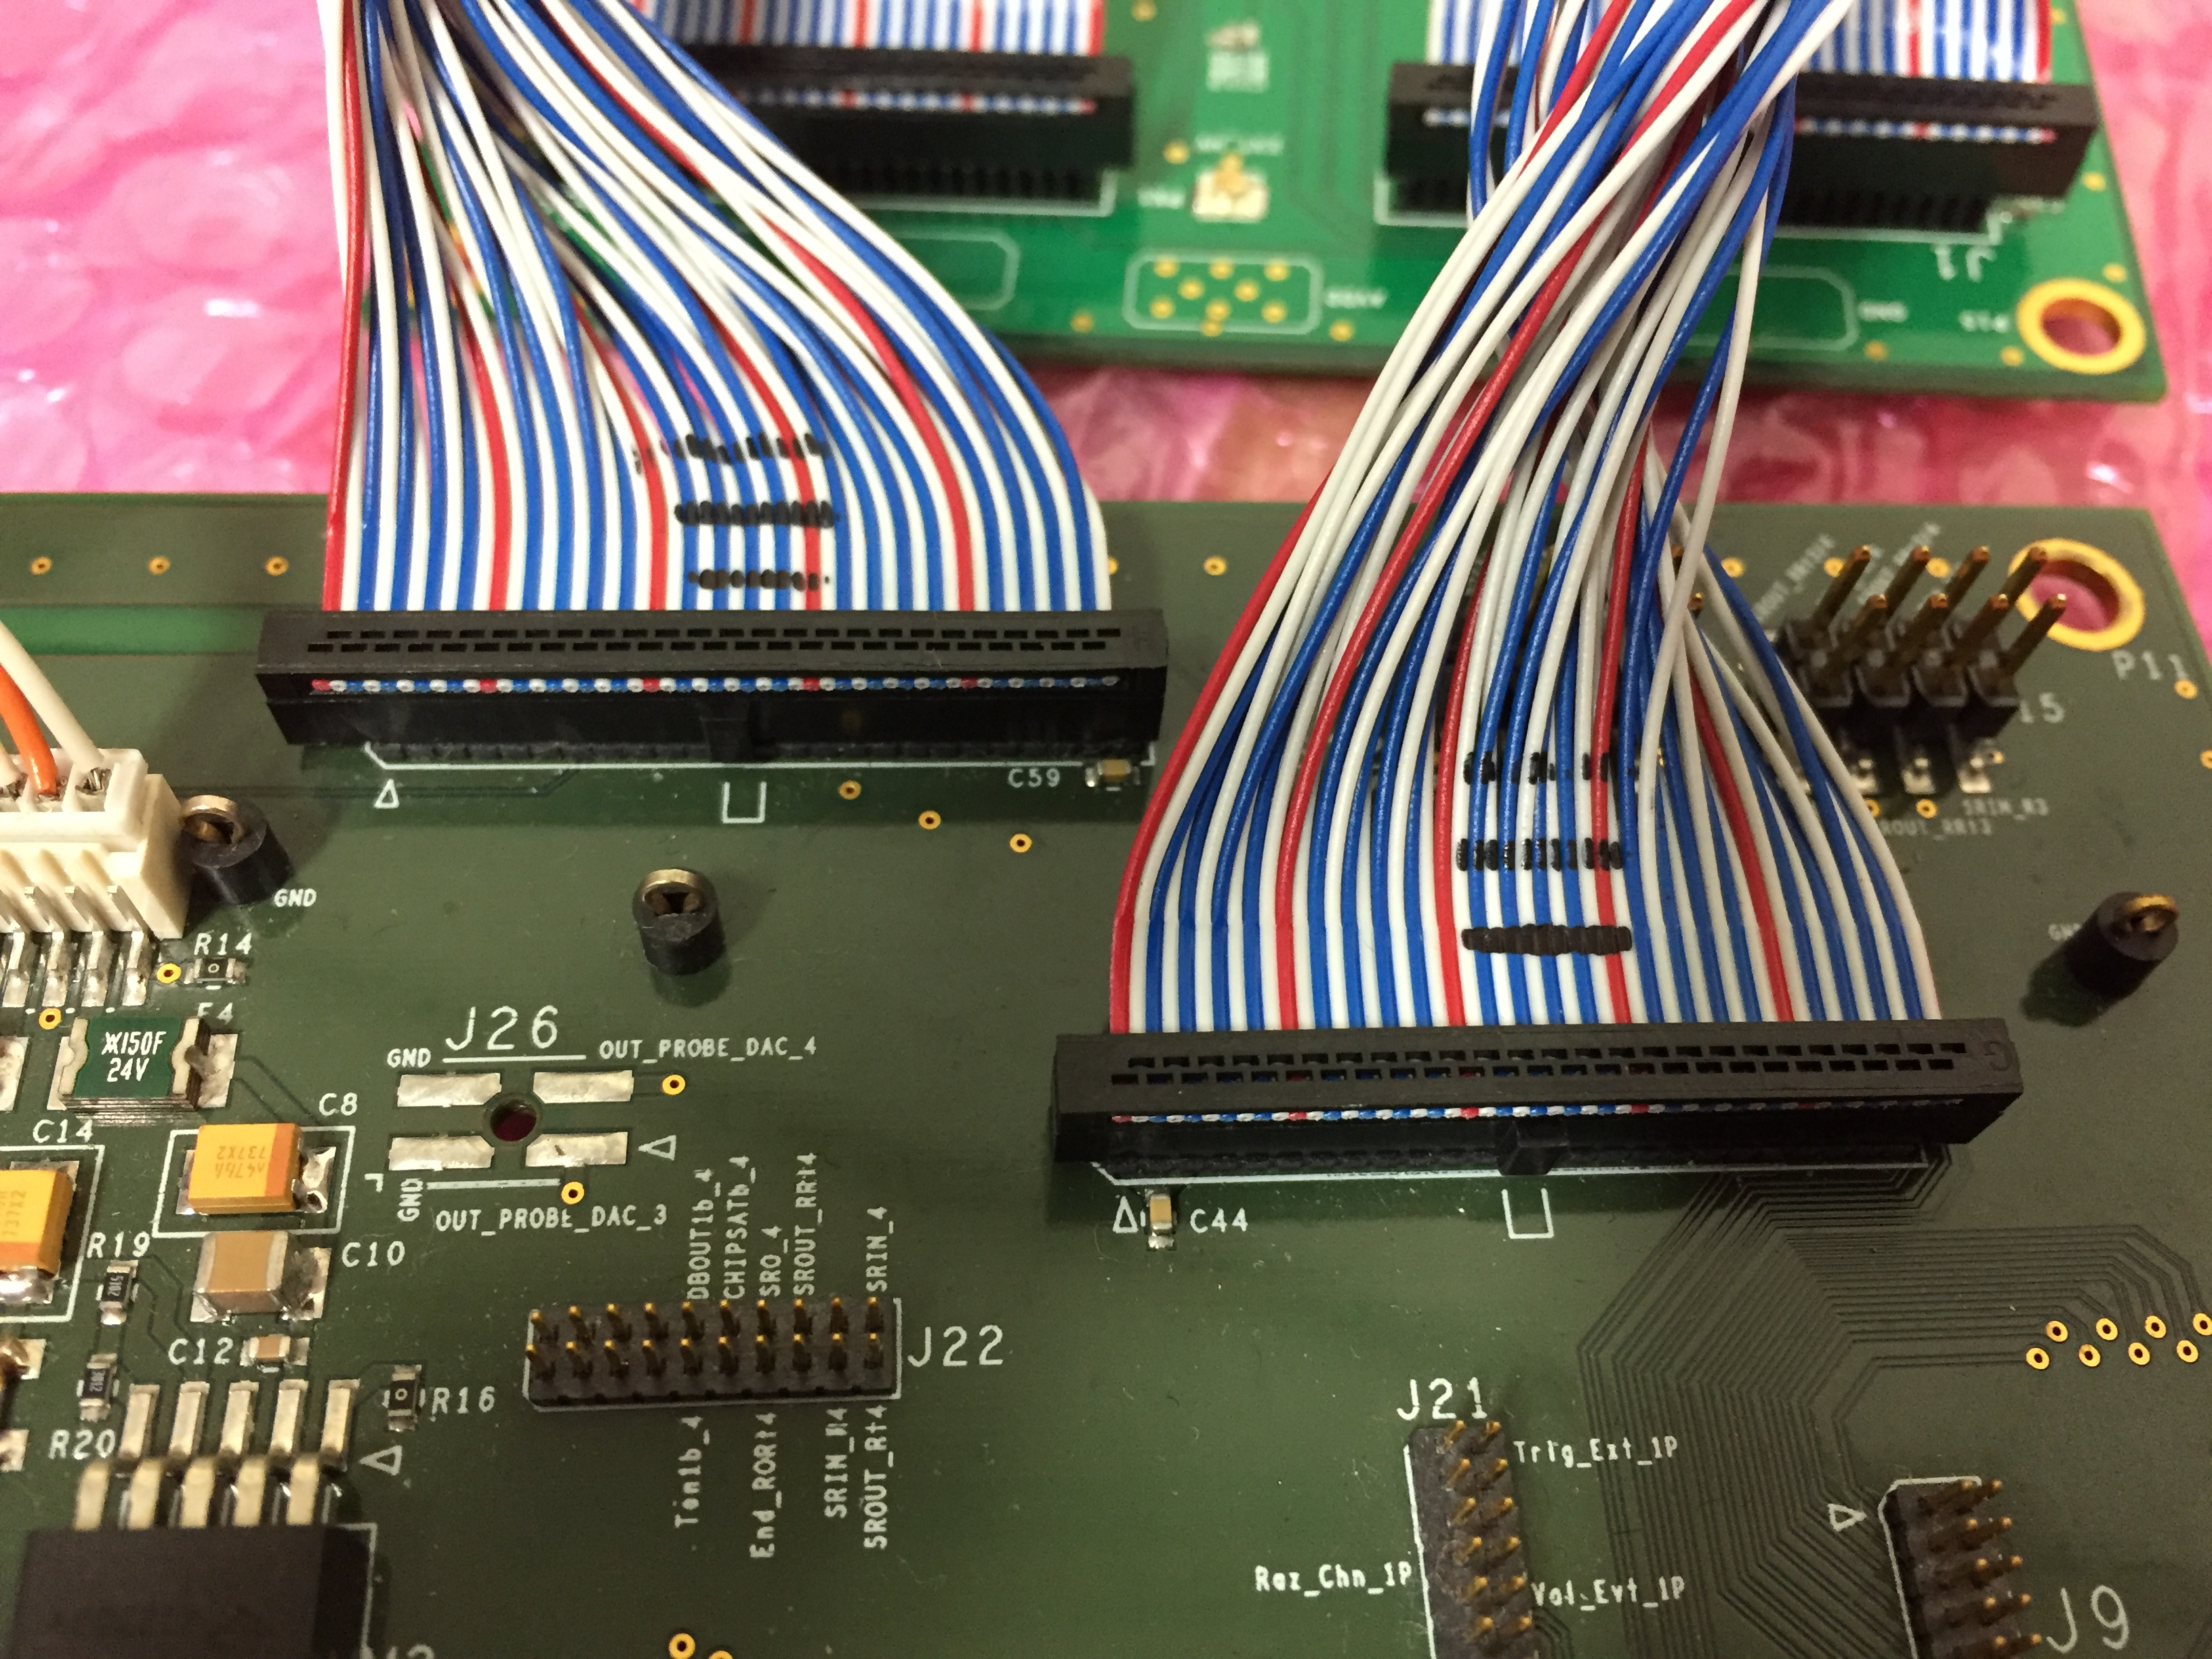
\includegraphics[width=0.9\linewidth,frame]{ASU-Interface2}
    \caption{Close view of the connectors}\label{fig:ASU-Interface2}
  \end{minipage}
\end{figure}
As can be seen in Figure~\ref{fig:ASU-Interface1}, depending on the relative
position and orientation of the ASUs and Interface, it can happen that the
cables cross. Notice also that the bump in the cable have to correspond to the
silkscreen prints on the circuit. Refer to table~\ref{tab:ASU-IF} for the ASU-IF
connections. The Jx mark is written on the PCB next to the relative connector,
where x is the connector number.
\begin{table}[H]
  \centering \bgroup
  \def\arraystretch{1.5}% 1 is the default, change whatever you need
  \begin{tabular}{|c|c|c|c|c|}
    \hline
    \textbf{Interface} & \textbf{ASU} \\
    \hline
    J2 & J1 (ASU1)  \\
    \hline
    J5 & J2 (ASU1)  \\
    \hline
    J6 & J1 (ASU2)  \\
    \hline
    J7 & J2 (ASU2)  \\
    \hline
    J8 & J1 (ASU3)  \\
    \hline
    J9 & J2 (ASU3)  \\
    \hline
    J10 & J1 (ASU4)  \\
    \hline
    J11 & J2 (ASU4)  \\
    \hline
  \end{tabular}
  \egroup
  \caption{ASU - Interface connections}\label{tab:ASU-IF}
\end{table}

\subsection{How to set the jumpers on the
  Interface}\label{sec:interface-jumpers}
Each interface can be connected to 4 ASU chains. Depending on how many chains
are to be connected, the Interface jumpers must be set appropriately. The
following four figures (\ref{readout_version_prod},
~\ref{srin_srout_version_prod},~\ref{srinread_sroutread_version_prod},
~\ref{start_end_readout_prod}) explain in detail which jumpers have to be
set. Refer to table~\ref{tab:IF-jumpers} for a summary of the pinout.
\begin{figure}[H] \centering
\includegraphics[width=0.8\linewidth]{readout_version_prod}
  \caption{}\label{readout_version_prod}
\end{figure}
\begin{figure}[H] \centering
\includegraphics[width=0.8\linewidth]{srin_srout_version_prod}
  \caption{}\label{srin_srout_version_prod}
\end{figure}
\begin{figure}[H] \centering
\includegraphics[width=0.8\linewidth]{srinread_sroutread_version_prod}
  \caption{}\label{srinread_sroutread_version_prod}
\end{figure}
\begin{figure}[H] \centering
\includegraphics[width=0.8\linewidth]{start_end_readout_prod}
  \caption{}\label{start_end_readout_prod}
\end{figure}
\begin{table}[H]
  \centering \bgroup
  \def\arraystretch{1.5}% 1 is the default, change whatever you need
  \begin{tabular}{|c|c|c|c|c|}
    \hline
    & \textbf{1 Chain (J2J5)} & \textbf{2 Chains (J2J5 and J6J7)} & \textbf{4 Chains} \\
    \hline
    \textbf{J12} & 1-2,3-4  & 1-2,4-6,7-8 & 1-2,4-6,8-10,12-14,16-18 \\
    \hline
    \textbf{J13} & 1-2,3-4  & 1-2,4-6,7-8 & 1-2,4-6,8-10,12-14,16-18 \\
    \hline
    \textbf{J15} & 1-2,3-4  & 1-2,4-6,8-18 & 1-2,4-6,8-10,12-14,16-18 \\
    \hline
    \textbf{J25} & no jumpers & 1-3 & 1-3,5-7,9-11 \\
    \hline
    \textbf{J26} & no jumpers & 1-3 & 1-3,5-7,9-11 \\
    \hline
    \textbf{J27} & no jumpers & 1-3 & 1-3,5-7,9-11 \\
    \hline
  \end{tabular}
  \egroup
  \caption{Interface jumpers. The dash '-' symbol indicates a direct connection
    of only two pins. So for example by 8-18 I mean connect pin 8 to pin 18 and NOT
    connect pin 8 to pin 9 to pin 10 to \dots to pin 18. The pin numbers are not
    written on the interface. Until now I have no idea of how to determine the pin
    numbers but to look at already jumper-ed Interfaces or from the following
    Figure~\ref{interface-jumpers}.}\label{tab:IF-jumpers}
\end{table}
\begin{figure}[H] \centering
  \includegraphics[width=0.8\linewidth]{interface-jumpers}
  \caption{Interface jumpers setup for 4 (all) ASU chains}\label{interface-jumpers}
\end{figure}

\subsection{How to patch the interface}\label{sec:how-patch-interface}
As can be read in Tamura Riku's thesis (after correcting some typos):

\textit{[\dots] in order to check the correct operation of the full setup, the
  daisy chain configuration is firstly tested. The test is done by increasing
  the number of daisy-chained ASU boards one by one. Up to about 10 boards, the
  daisy chain is correctly configured but at around 10 boards the configuration
  starts to fail. After several tests with different configurations, it appeared
  that this is due to the attenuation and reflection of the bunch crossing clock
  (BCID) when it travels through the chain: the signals, including the bunch
  crossing clock, are serially transported through the daisy chain so the length
  that they need to travel depends on the number of connected ASU boards. The
  total capacitance of the daisy chain depends on the number of connected ASU
  boards, too. This creates a mismatch of impedance between the endpoints and
  some DAQ signals are badly affected. In practice most of the DAQ signals are
  not so affected but it seems that the bunch crossing clock is strongly
  affected. The whole DAQ acquisition phase is synchronized to the bunch
  crossing clock so this is a very critical issue.}

\textit{Fortunately, this problem can be fixed by ``patching'' the bunch
  crossing clock line. To prevent the attenuation of bunch crossing clock and
  match the impedance a 4ch buffer,
  CDCLVC1104\cite{Texas-Instruments:CDCLVC11xx}, is applied to the bunch
  crossing clock line as shown in Figure TO-DO. This buffer is a highly
  performing and fast responding one. The delay it adds to the BCID is of
  0.8-2ns, which is less than 1\% of the period of bunch crossing clock, so the
  effect on the timing measurement due to the BCID is negligible. This patch is
  tested to work fine and the daisy chain is configured correctly even with the
  full setup (20 ASUs). [\dots]}

Long story short, we have to patch every interface with that chip if we want to
daisy-chain more than 10 ASUs. Just to be on the safe side, all the interface
boards, even if connected to less than 10 ASUs, were fixed with the following
procedure.
\begin{figure}[H]
  \centering \includegraphics[width=.8\textwidth]{buffer-role}
  \caption{Cartoonist impression of the reason why we need to patch the
    Interface with a buffer chip.}\label{fig:buffer-role}
\end{figure}

Here I will show how to concretely fix the interface. I came to know about this
procedure by reading two pdf files that were sent to YNU from I don't know
where. I must admit that until now they hold the record for being the most
unintelligible piece of paper that I have ever read. No matter how much I
strove, I think that I could never write in such a cumbersome manner even if I
want to. Anyway \dots
\begin{enumerate}
\item First solder the CDCLVC1104 chip on the base and glue it on the board (any
  empty space on the interface is good) as shown in Figure~\ref{buffer}. You can
  use a different support (the white piece of plastic) and base (the small PCB
  with 10 holes on each side) if you want.
  \begin{figure}[H]
    \centering \includegraphics[frame,width=.3\textwidth]{support}\hfill
    \includegraphics[frame,width=.3\textwidth]{base}\hfill
    \includegraphics[frame,width=.3\textwidth]{base-glued}
    \caption{PCB Base (in the middle) glued to the interface board using a
      plastic support (on the left). The buffer chip must be soldered on that
      base (not shown in the pictures, yet). You can solder the buffer chip in
      any position on the base as long as it is soldered
      properly.}\label{buffer}
  \end{figure}
\item Then take a 50 pins flat cable (that you are then going to connect to the
  J2 connector). Cut in the middle the wires number 13, 49 and 50 (SR\_CK\_BUF,
  TRIG\_EXT\_N and TRIG\_EXT\_P respectively). Refer to Figure~\ref{J2} for the
  flat cable pin-out. Strip the ``ASU end'' of these wires. By ASU end I mean
  the end that is not to be connected to the interface but to the ASU. If needed
  do the same for the other flat cables coming out the connectors J6, J8 and
  J10.
  \begin{figure}[H]
    \centering \includegraphics[frame,width=0.7\linewidth]{J2}
    \caption{J2 connector pin-out}\label{J2}
  \end{figure}
\item Desolder the M9 chip
  \begin{figure}[H]
    \centering \includegraphics[frame,width=0.5\linewidth]{desolder}
    \caption{CDCLVC1104 chip pin-out}\label{desolder}
  \end{figure}
\item Referring to Figures~\ref{interface-connections}
  and~\ref{buffer-blueprint}, connect with some wires the pins in this way:
  \begin{table}[H]
    \centering \bgroup
    \def\arraystretch{1.5}% 1 is the default, change whatever you need
    \begin{tabular}{|c|c|c|}
      \hline
      \textbf{color} & \textbf{CDCLVC1104 pin} & \textbf{Interface pin} \\
      \hline
      brown & 1 CLKIN & SR\_clk \\
      \hline
      red & 6 VDD & (refer to picture) \\
      \hline
      black & 4 ground & Interface ground \\
      \hline
    \end{tabular}
    \egroup
    \caption{Fast command packet format}
  \end{table}
  \begin{figure}[H]
    \centering \includegraphics[width=0.7\linewidth]{buffer-blueprint}
    \caption{CDCLVC1104 chip pin-out}\label{buffer-blueprint}
  \end{figure}
  \begin{figure}[H]
    \centering
    \includegraphics[frame,width=.3\textwidth]{interface-pinout1}\hfill
    \includegraphics[frame,width=.3\textwidth]{interface-pinout2}\hfill
    \includegraphics[frame,width=.3\textwidth]{ground}
    \caption{Interface connections}\label{interface-connections}
  \end{figure}
  I am sorry but in the document that I was given there is no schematics
  regarding the holes around the M9 chip, so we had to solder referring only to
  the attached pictures.
\item (Optional but recommended) Solder a capacitor of 100nf to decouple power
  and ground between the pins 6 VDD and 4 GRD of the buffer. It is not shown in
  the pictures.
\item Now connect the interface holes around the M9 chip as shown in
  Figures~\ref{interface-connections} (blue cable). In the document I was given
  those are called pin number 1 and 7. Anyway, as I said, without the schematics
  those numbers are meaningless. Sometimes I wonder if Physicists are really so
  smart as they think to be.
\item Pins 3,5,7,8 of the buffer chip represent the output of the
  buffer. Connect each pin to the wire number 13 of the flat cables coming off
  J2, J6, J8 and J10. The order is not relevant. Of course, in the case of the
  SideMRD, only one connection is needed (for example J2). Refer to
  Figure~\ref{connection_flat_cable_1} for a visual explanation.
  \begin{figure}[H]
    \centering \includegraphics[width=0.6\linewidth]{connection_flat_cable_1}
    \caption{How to connect the \#13 wire to the buffer.}%
    \label{connection_flat_cable_1}
  \end{figure}
\item Connect wire number 50 of the flat cable (it is white in our case) to any
  ground pin on the interface board. You have to connect the ``ASU end'' of the
  wire to ground in a similar way as shown in Figure~\ref{connection_flat_cable_2}
  for the case of cable 13.
    \begin{figure}[H]
    \centering \includegraphics[width=0.6\linewidth]{connection_flat_cable_2}
    \caption{How to connect the \#49 and \#50 wires to the DVDD and Ground pins.}%
    \label{connection_flat_cable_2}
  \end{figure}
\item Connect wire number 49 of the flat cable (it is blue in our case) to the
  DVD pin on the interface board. The DVDD pin is located near the M9 chip that
  you just desoldered. You have to connect the ``ASU end'' of the wire to the
  DVD pin in a similar way as shown in Figure~\ref{connection_flat_cable_2} for
  the case of cable 13.
\item The final result should look more or less like
  Figure~\ref{fixed-interface}.
  \begin{figure}[H]
    \centering 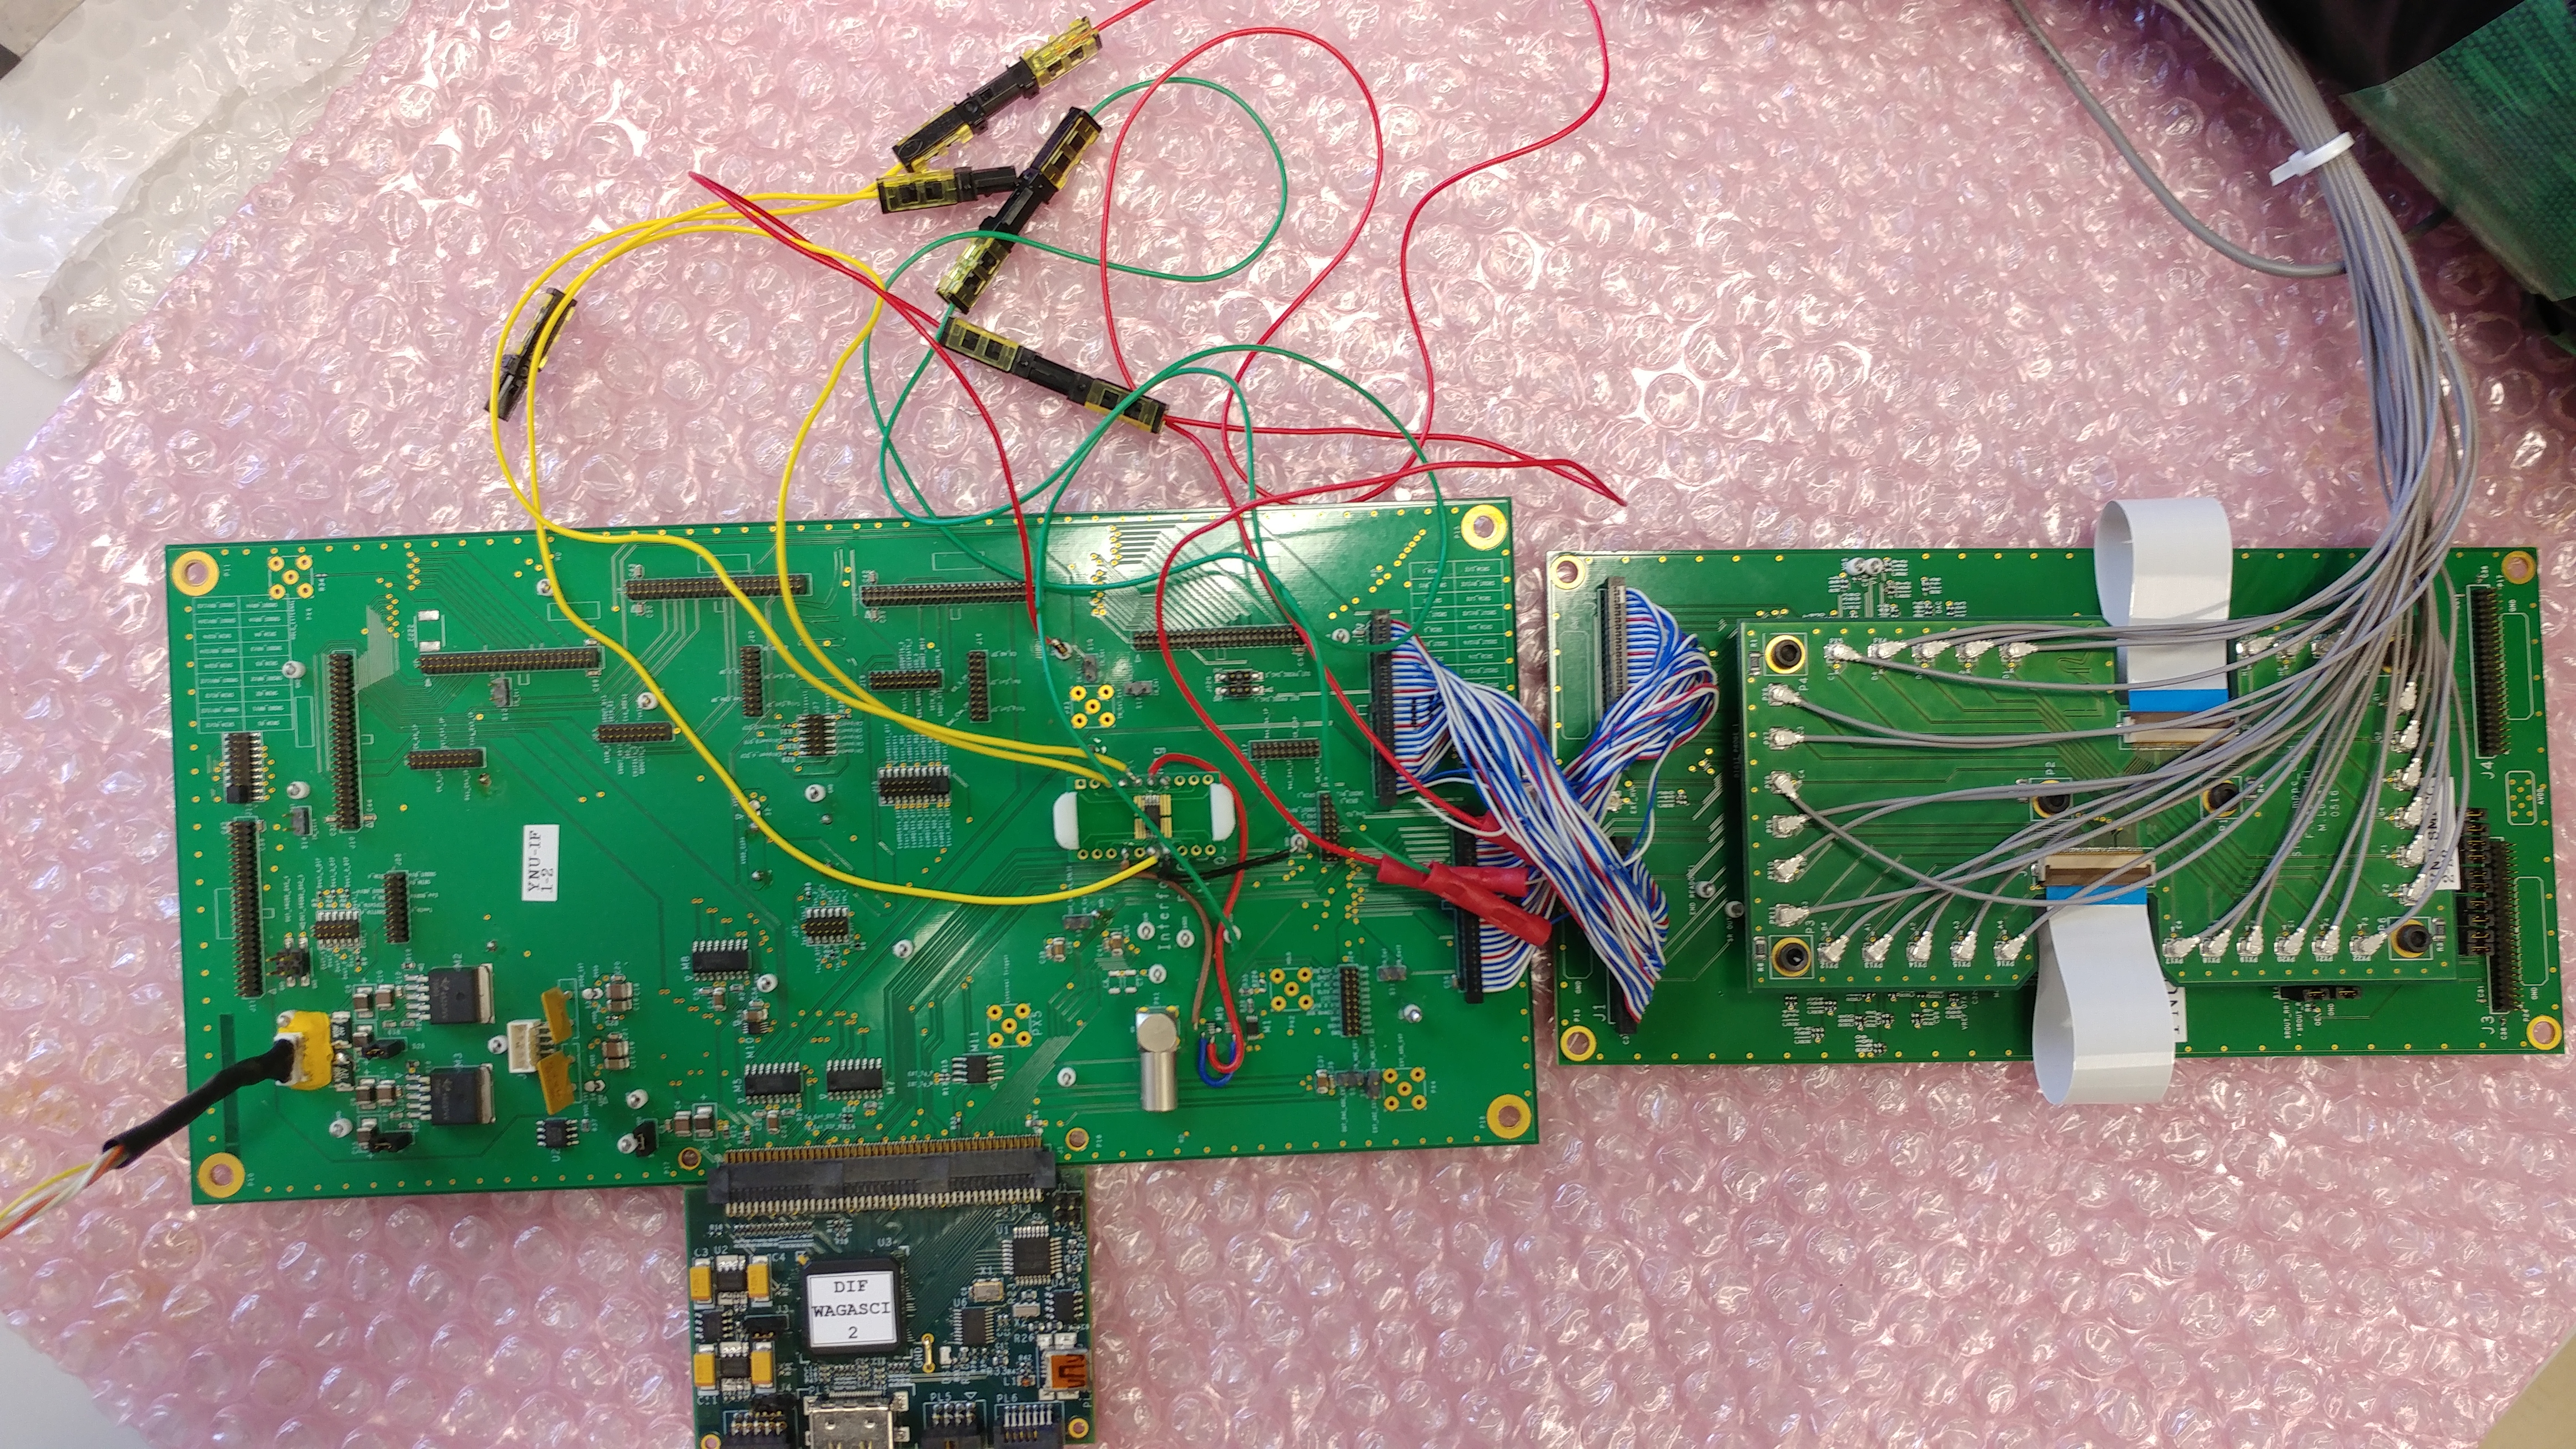
\includegraphics[frame,width=0.9\linewidth]{fixed-interface}
    \caption{Final result. The ground wire coming from wire 50 of
      the flat cable is red (sorry for the ambiguity). The green
      wire is coming off from wire number 49 and is connected to the DVD pin on
      the Interface. In total there are three yellow output wires coming off the
      buffer chip but only one is actually used.}\label{fixed-interface}
  \end{figure}
\end{enumerate}

\subsection{How to make a Low Voltage cable}\label{sec:how-make-low-voltage-cable}
For bench-testing purposes you may need to make your own Low Voltage cable to
power the Interface and all the other boards connected to it.

The Low Voltage cable must be connected to the interface using a 5 pins
connector to a vertical wire-to-board socket that looks like this:
\begin{figure}[H]
  \centering
  \begin{minipage}{0.15\linewidth}
    \centering \includegraphics[width=\linewidth,frame]{low-vol-socket1}
  \end{minipage}%
  \begin{minipage}{0.6\linewidth}
    \centering \includegraphics[width=0.9\linewidth,frame]{low-vol-socket2}
  \end{minipage}
  \caption{Vertical wire-to-board 5-pins socket on the Interface board for the
    Low Voltage connection}\label{low-vol-socket}
\end{figure}
To make the cable just buy a male connector (TO-DO insert link) and connect the
pins following the pin-out of Figure~\ref{low-vol-pin-out}.
\begin{figure}[H]
  \centering \includegraphics[width=0.5\linewidth]{low-vol-pin-out}
  \caption{Vertical wire-to-board 5-pins socket on the Interface board for the
    Low Voltage connection}\label{low-vol-pin-out}
\end{figure}
The ground wires can be grouped together in a single wire. The 5V wires can be
grouped together in a single wire, too. The resulting 2 wires end of the cable
can be terminated as you like and then connected to a 5V power supply. The power
supply should be able to generate at least TO-DO Amperes of current.

\section{DIF}
I have not much to say about the Detector InterFace (DIF) board. It converts the
signal from the ASUs into HDMI and sends it to the GDCC. It also controls the
synchronization and reset of the slow clock (BCID). Until present there were
many issues related to the slow-clock reset and synchronization, all of which
have been luckily solved by a DIF firmware upgrade. To know more about the DIF
please contact Matsushita Kouhei (Tokyo University): he was the one that tested
the new firmware. To flash the updated firmware refer to Section TO-DO

Remember to note down the port number (Figure~\ref{fig:GDCC-front-view}) on the
GDCC side that you connect each DIF to, because you will have to insert that
number in the configuration file TO-DO.
\begin{figure}[H]
  \centering
  \begin{minipage}{0.2\linewidth}
    \centering \includegraphics[width=0.9\linewidth, frame]{GDCC-front-view}
    \caption{GDCC front view}\label{fig:GDCC-front-view}
  \end{minipage}%
  \begin{minipage}{0.7\linewidth}
    \centering \includegraphics[width=0.9\linewidth, frame]{DIF}
    \caption{Detector InterFace (DIF)}
  \end{minipage}
\end{figure}

\subsection{DIF Firmware upgrade}
Refer to table~\ref{table:dif-firmware} for the list of needed parts.
\begin{table}[H]
  \centering
  \begin{tabular}{|l|l l l l l l l l l|}
    \hline
    \textbf{Connector on DIF} & \textbf{1} & \textbf{2} & \textbf{3} %
    & 4 & 5 & \textbf{6} & \textbf{7} & \textbf{8} & NC \\
    \textbf{Connector on Housing} & \textbf{1} & \textbf{2} & \textbf{3} %
    & NC & NC & \textbf{4} & \textbf{5} & \textbf{6} & NC\\
    \textbf{Xilinx USB cable} & \textbf{TCK} & \textbf{GND} & \textbf{TMS} %
    & NC & NC & \textbf{TDI} & \textbf{TDO} & \textbf{VREF} & NC \\
    & (Yellow) & (Black) & (Green) & & & (White) & (Purple) & (Red) & (Gray) \\
    \hline
  \end{tabular}
  \caption{Pinout for the TDK-Lambda ZUP6-33 LV PSU}
\end{table}

\section{GDCC}
\begin{figure}[H]
  \centering \includegraphics[width=0.7\linewidth, frame]{GDCC}
  \caption{Gigabit Data Concentrator Card (GDCC) or Clock and Control Card
    (CCC)}
\end{figure}
I have not much to add in addition to what is already in the literature quoted
in Section~\ref{sec:overview}. This is the board that I know the least about,
just because, fortunately, it just works and has never given any problem so far.

Please refer to the literature~\cite{GDCC:2012} or
Appendix~\ref{sec:gdcc-cheat-sheet} if you want/need to know more about the
GDCC.

The communication between the PC and GDCC is built on standard
Ethernet. Communication to and from it is done via RAW Ethernet packets. This is
why it doesn't need an IP address. This way communication between the DAQ PC and
the GDCC can be faster than if they traveled through the IP layer but the GDCC
must necessarily be located on the same physical LAN network as the DAQ PC.

The GDCC communicates with the ZedBoard using raw Ethernet packets. This
connection is through ``Normal GDCC packets'': \cleanstyle{0x0810}
(Appendix~\ref{sec:gdcc-cheat-sheet}).

\subsection{How to make a power supply cable}
The GDCC is build in the standard VME layout. It is meant to be plugged into a
VME crate slot for power and mechanical stability. As far as I know,
communication with the VME crate is hardware-ready but not implemented in
software yet.

In case you don't have a VME crate at hand you can easily fabricate a specific
power adapter to power up the GDCC and CCC with a standard Power Supply
Unit. The nominal voltage is DC $+5V$. The PSU must be able to supply at least
$5A$ of DC current.

For this, you need to find or buy
\begin{itemize}
\item 2 VME female connectors (96 way 2.54mm pitch). One for the GDCC and
  another for the CCC (RS reference number:
  \href{https://jp.rs-online.com/web/p/din-41612-connectors/0470443/?sra=pstk}{RS
    470-443}).
\item A breadboard to solder the connectors and the cables onto (RS reference
  number in Europe
  \href{https://uk.rs-online.com/web/p/matrix-boards/4570755/}{RS 457-0755}, RS
  reference number in Japan
  \href{https://jp.rs-online.com/web/p/matrix-boards/6647876/?sra=pstk}{RS
    664-7876}) (single side Matrix board, 2.54 pitch). You need only one boards
  that you can cut in 2 parts, one for each adapter.
\item Black and red cable unipolar cable for connections.
\item Two connectors to connect to the Power Supply (the connector type depends
  on your Power Supply and your ``taste'').
\end{itemize}

In the following I will show how to concretely make the said cable using a hot
air station and soldering iron. You don't necessarily need a hot air station and
you can get the same result with only a soldering iron and a bit of
patience. The following pictures refer to two cables made with slightly
different techniques, so some minor details can differ between the pictures.

\begin{enumerate}
\item First cut the breadboard in the desired shape. As long as the cut
  breadboard doesn't hinder the two VME connectors from fitting one into the
  other, any shape is fine.
\item Then apply the solder paste evenly on the breadboard surface and insert
  the female connector. I have used two copper wires for the ground connections,
  but any other solution to make the connections is fine.
  \begin{figure}[H]
    \centering \includegraphics[width=0.7\linewidth,
    frame]{power-connector-solder-paste}
  \end{figure}
\item Solder all the pins using the hot air station (I recommend a air
  temperature of 370 degrees Celsius)
  \begin{figure}[H]
    \centering 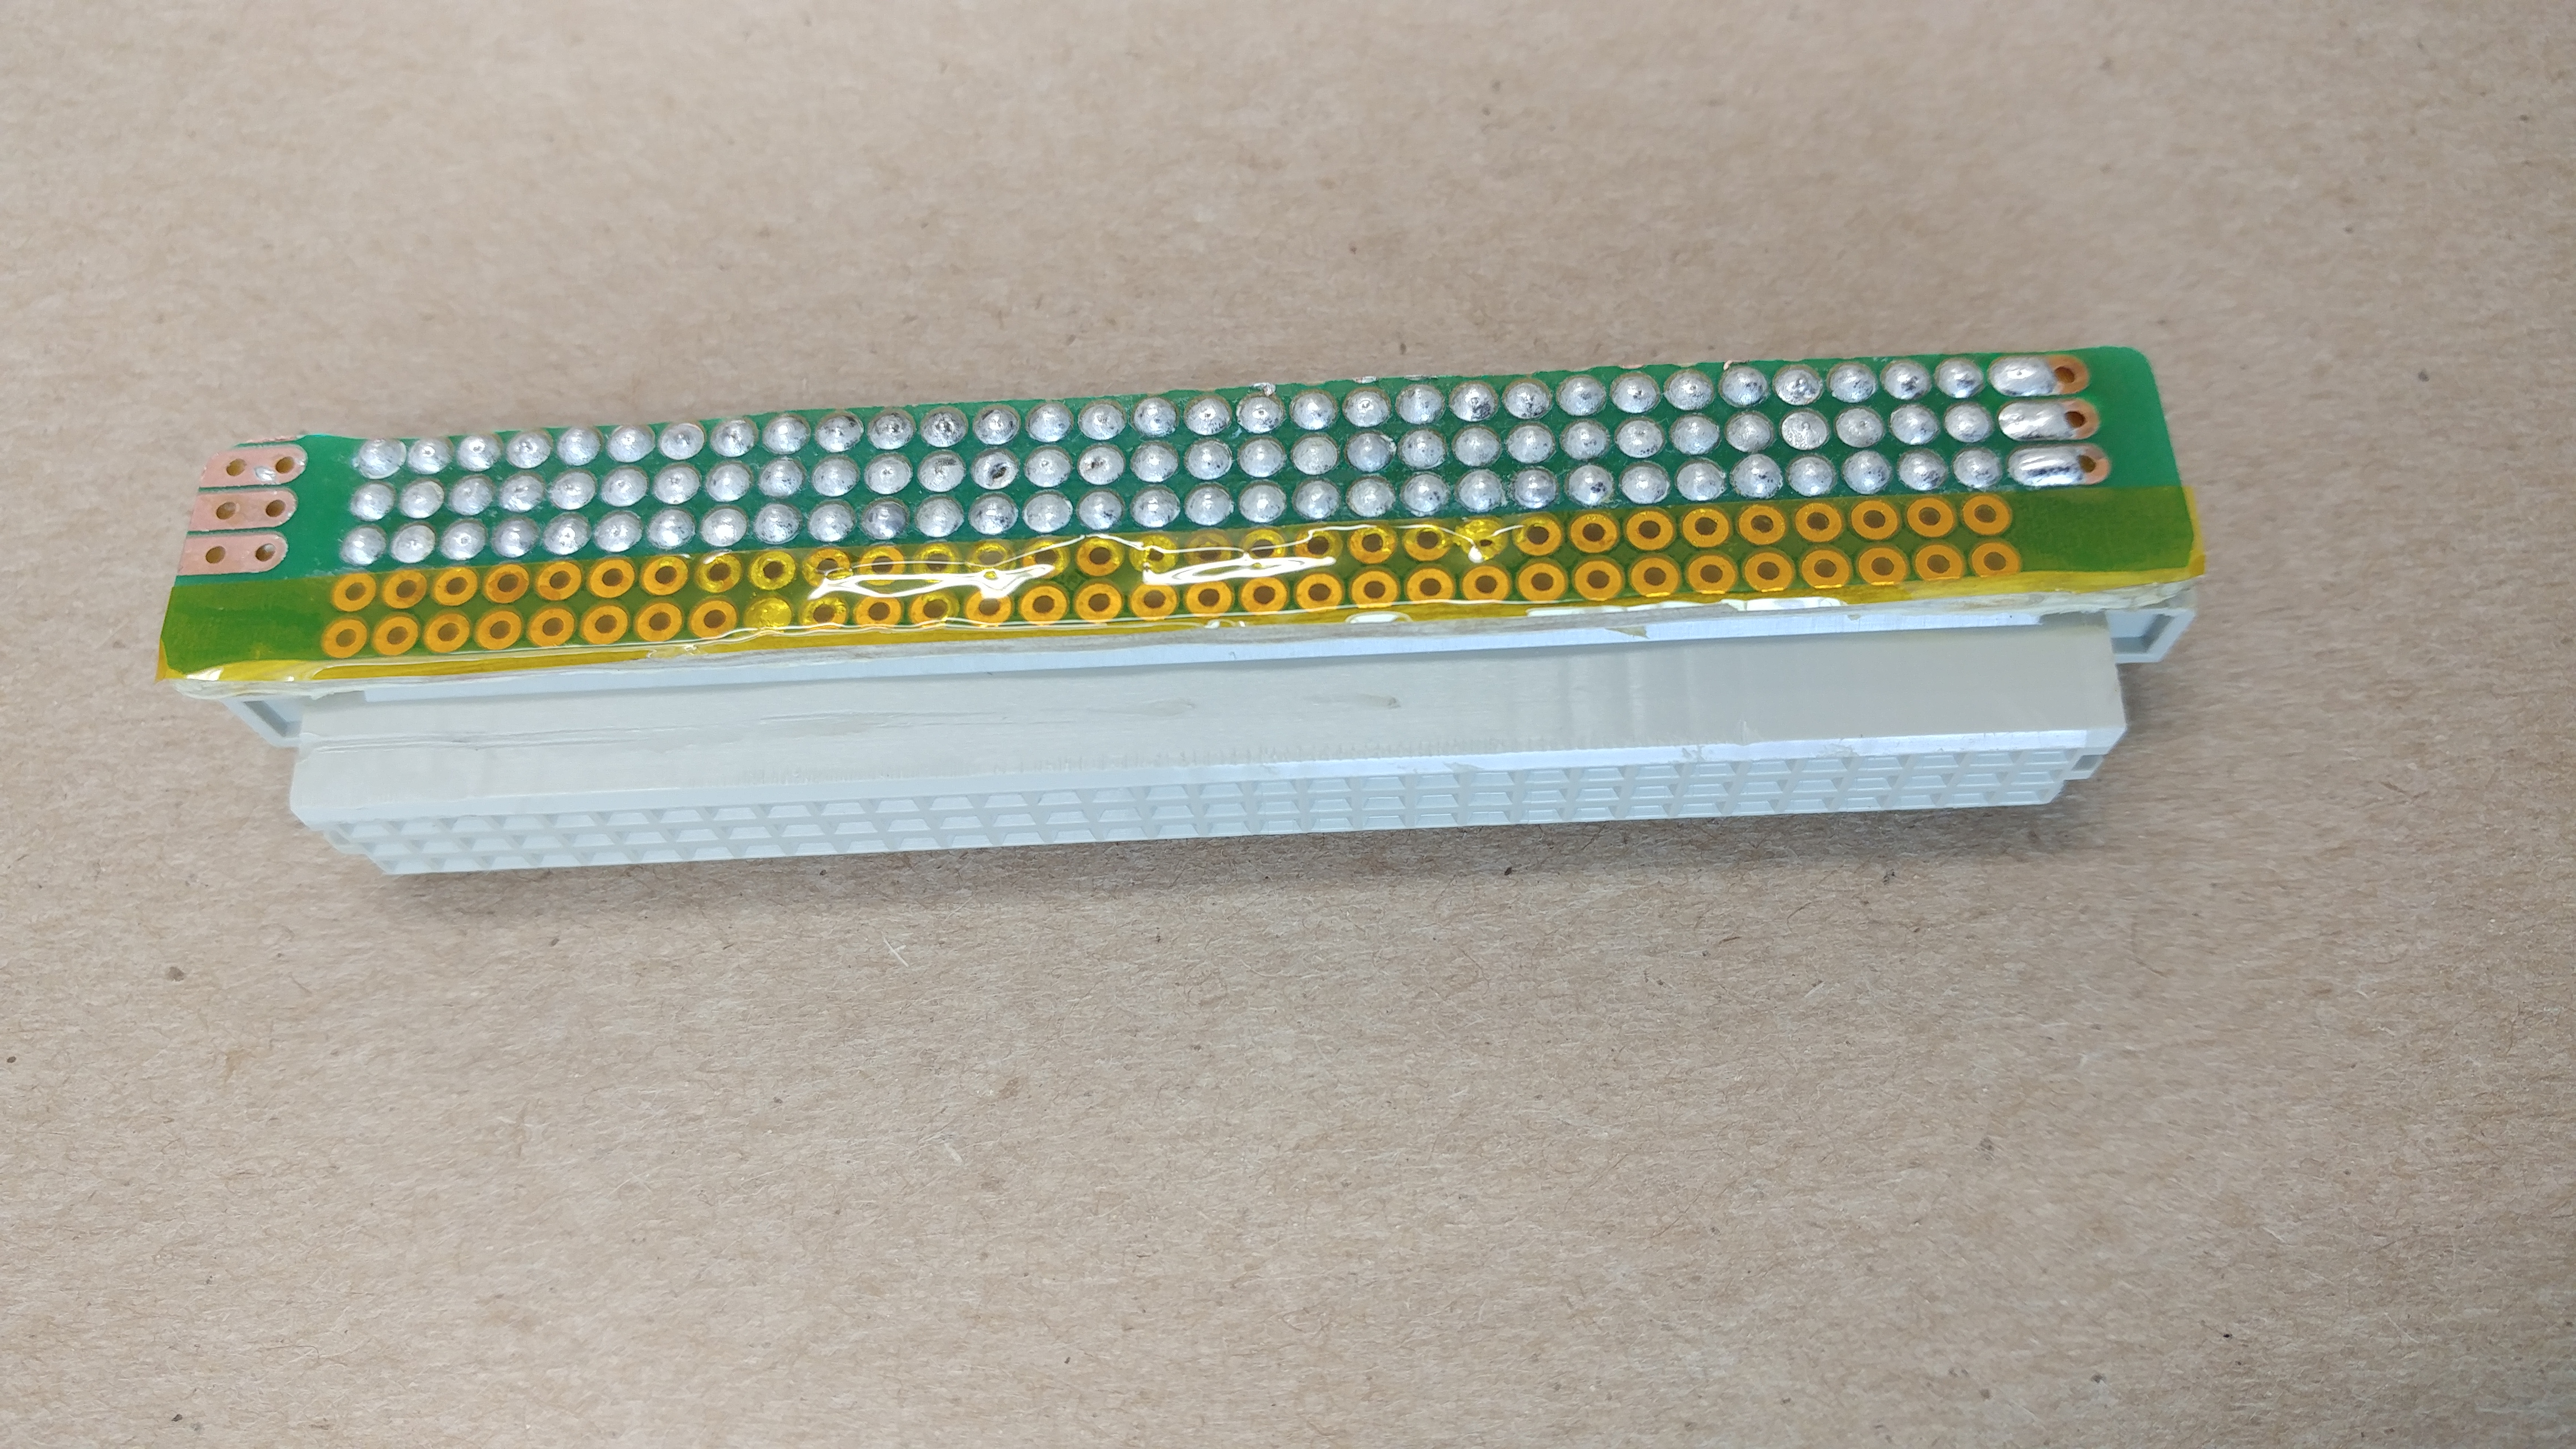
\includegraphics[width=0.7\linewidth,
    frame]{power-connector-hot-air}
  \end{figure}
\item Solder the pins A32, B32, C32 together and connect these one to a red
  cable that you will then use for the 5V voltage.  Then solder the pins A9,
  A11, A15, A17, A19, B20, B23, C9 together and connect these ones to a black
  cable that you will then use for the ground. To identify these pins you have
  first to identify the rows (A,B,C) and columns (1,2,\dots,31,32) of your
  connector. As explained before, you have to use a standard 3 rows, 92 pins VME
  female connector. This connector must have three rows labeled A, B and C and
  32 pins for each row labeled 1,2,\dots,31,32, for a total of 96 pins. Don't
  look at whatever may it written on the adapter itself or on the internet
  because it might be different from the GDCC or CCC specifications (as happened
  to me). Just take a look at the GDCC and in particular at the silkscreen near
  the VME connector. As shown in the next picture, look for the C1 and C32
  labels next to the respective pins. In the picture is also shown how to
  identify the A, B and C rows.
  \begin{figure}[H]
    \centering \includegraphics[width=0.48\linewidth,
    frame]{power-connector-connector}\hfill
    \includegraphics[width=0.48\linewidth, frame]{power-connector-connections}
  \end{figure}
  Then solder two long-ish wires for connecting the +5V and ground to a power
  supply and you cables are ready.
  \begin{figure}[H]
    \centering \includegraphics[width=0.48\linewidth,
    frame]{power-connector-cable-1}\hfill \includegraphics[width=0.48\linewidth,
    frame]{power-connector-cable-2}
  \end{figure}
\end{enumerate}


\section{CCC}
Clock and Control Card (CCC). It is used to process the beam trigger signal
(Section~\ref{sec:beam-trigger-spill}), to create the spill flag variable, TO DO\dots

To communicate with the PC it uses the SiTCP hardware and protocol~\cite{Uchida:2008}
with a fixed IP address of \cleanstyle{192.168.10.2}.
\subsection{How to convert a GDCC into a CCC}
\epigraph{Do you know how the Orcs first came into being? They were elves once,
  taken by the dark powers. Tortured and mutilated: a ruined and terrible form
  of life.}{The Lords of the Rings} All the CCC boards are produced as GDCC and
then converted in CCC by flashing a new firmware and slightly modifying the
printed board. The modification is not so complex and with a minimum effort can
be done by hand if one has the right tools.

To flash the firmware you need a Xilinx programmer like this: TO-DO

Once the firmware has been flashed it is time to modify the printed circuit. You
only need to short the R28 and R29 resistors by inserting two $0\Omega$ resistor
in the appropriate pins.
\begin{figure}[H]
  \centering \includegraphics[width=0.5\linewidth,frame]{GDCC-CCC1}
  \caption{The position of the R28 and R29 resistors on the board.}
\end{figure}
\begin{figure}[H]
  \centering \includegraphics[width=0.8\linewidth]{GDCC-CCC2}
\end{figure}
You can solder the resistors with a traditional solder iron or with a hot air
gun. In any case you need at least two $0\Omega$ resistors of size 1608 (1.6 mm
× 0.8 mm). You can find them on the Japanese RS web-shop under the RS reference
number ``631-5667''. The full description is:
\begin{itemize}
\item \begin{CJK}{UTF8}{min}KOA 厚膜チップ抵抗器,ジャンパーチップ抵抗器, 1608サイ
    ズ, $0\Omega$, $\pm
    0$ \\
    RS品番 631-5667 メーカー型番 RK73Z1JTTD メーカー/ブランド名 KOA\end{CJK}
\item KOA thick-film resistor, jumper-chip resistor, size 1608, $0\Omega$, $\pm
  0$ \\
  RS number 631-5667 maker number RK73Z1JTTD maker/brand KOA
\end{itemize}
Anyway, the maker is not important as long as the value and size are correct.
You can solder the resistor in at least two ways. One is with a soldering
conical tip
\begin{itemize}
\item iron soldering you will also need:
  \begin{itemize}
  \item solder (remember that lead is poisonous for all life forms including
    you)
  \item tweezers
    (\href{https://www.monotaro.com/p/0840/4873/?displayId=5}{monotaro number
      TSP-26})
  \item flux (\href{https://www.monotaro.com/p/3952/8833/?displayId=5}{monotaro
      number FS20001})
  \item flux remover
    (\href{https://www.monotaro.com/p/6215/1382/?displayId=5}{monotaro number
      BS-W20B})
  \end{itemize}
\item hot air gun soldering
  (\href{https://www.monotaro.com/p/4893/0954/?displayId=5}{monotaro number
    FR810B-81}) you will also need:
  \begin{itemize}
  \item solder paste (it already contains flux)
    (\href{https://www.monotaro.com/p/1001/3097/?displayId=5}{monotaro number
      SMXB05})
  \item tweezers
  \item flux remover
  \item heat resistant tape
    (\href{https://www.monotaro.com/p/5638/8526/?displayId=5}{monotaro number
      15})
  \end{itemize}
\end{itemize}

\section{Low and High Voltage PS}
\subsection{TDK-Lambda ZUP6-33}
\begin{table}[H]
  \centering
  \begin{tabular}{|l|l l l l l|}
    \hline
    \textbf{Signal} & \textbf{GND} & \textbf{5.0V}
    & \textbf{GND} & \textbf{5.0V} & \textbf{GND} \\
    \hline
    Molex on IF & 1 & 2 & 3 & 4 & 5 \\
    Feed-through connector & 1 & 2 & 3 & 4 & 5 \\
    Terminal on LV PSU & 2 & 1 & 2 & 1 & 2 \\
    \hline
  \end{tabular}
  \caption{Pinout for the TDK-Lambda ZUP6-33 LV PSU}
\end{table}

\subsection{HV PSU: TDK-Lambda ZUP80-2.5}
\begin{table}[H]
  \centering
  \begin{tabular}{|l|l l l|}
    \hline
    & \textbf{LEMO} & \textbf{SHV} & \textbf{DSUB} \\
    \hline
    Signal & Central conductor & Pin & 1 \\
    NC &  &  & 2 \\
    GND & Outer shield & GND Lug Terminal & 3 \\
    \hline
  \end{tabular}
  \caption{Pinout for the TDK-Lambda ZUP80-2.5 LV PSU}
\end{table}

\subsection{HV PSU: Keithley 2400 SourceMeter}
From the Keithley 2400 SourceMeter manual:\textit{The Keithley 2400 SourceMeter
  combines a precise, low-noise, highly stable DC power supply with a low-noise,
  highly repeatable, high-impedance multimeter.}

I used this device at Yokohama National University as a High Voltage source for
my tests. This section describes how to operate this instrument from a personal
computer. Why go through the hassle of operating the Keithley from remote, if
every operation can be also performed directly from the detector front panel?
you may ask \dots The fact is that, back then, I was still in the process of
learning the Pyrame framework and I though that writing the Pyrame interface for
this instrument could be a good chance to test my comprehension of the Pyrame
code. Anyway, you may skip this section if you don't own a Keithley 2400 or you
are not interested in remotely operating it.

\subsubsection{GPIB or RS-232?}
You can connect the Keithley 2400 to a PC in two ways, each one with pros and
cons. One way is by using the GPIB port and the other is by using the RS232
port.
\begin{figure}[H]
  \centering \includegraphics[width=0.7\linewidth]{keithley-2400-rear-panel}
  \caption{The Keithley 2400 SourceMeter rear panel.}\label{keithley-2400-rear-panel}
\end{figure}

The General Purpose Interface Bus (GPIB but also called IEEE-488) is a
short-range bus specification. Newer standards have largely replaced GPIB for
computer use, but it still sees some use in the test equipment field. There are
GPIB drivers for linux but they are not usually included in most distributions
repositories, so you may have to compile them yourself. Since the WAGASCI DAQ
runs on Linux I am not considering here Windows and Apple. For example, you can
find a binary package for CentOS 7 ready to install but, in the case of Ubuntu,
you have to compile it from source yourself.

To physically connect the instrument you have three options: a GPIB-to-USB
adapter, a GPIB-to-Ethernet adapter or a PCI-GPIB board. I have personally
tested only the GPIB-to-USB adapter case. The main problem with GPIB is that in
any case, it is very expensive. The average price for any of those adapters is
around 200\$ or 20000¥ on Amazon (probably much more on specialized sites).
\begin{itemize}
\item GPIB pros
  \begin{itemize}
  \item You don't need to worry about the cable pinout
  \item Adapters and cables are quite standardized so every cable and adapter
    will work just fine.
  \end{itemize}
\item GPIB cons
  \begin{itemize}
  \item You need an adapter or a PCI-GPIB card
  \item It is very expensive (both cables and adapters)
  \item It requires you to install or compile specialized drivers
  \item If you use a GPIB-to-USB adapter you are limited to 3 meters for the
    length of the USB cable
  \end{itemize}
\end{itemize}

In the case of RS-232, only a simple serial cable with DB-9 connectors is needed.
\begin{itemize}
\item RS-232 pros
  \begin{itemize}
  \item It doesn't require a specialized adapter (or a very cheap one)
    since virtually any Desktop motherboard already have a serial port (called
    sometimes COM port).
  \item Cables and adapters are quite cheap. In the case of a Desktop PC you
    can get by with very little money (20\$ or 2000¥).
  \item It doesn't required specialized drivers
  \end{itemize}
\item RS-232 cons
  \begin{itemize}
  \item Choosing the right cable and adapter is difficult because there are so
    many different types of RS-232 cables.
  \item You may need to refer to your motherboard and to the Keithley serial
    port pinout schematics to understand which is the right cable/adapter or to
    fix the adapter pinout if you bought the wrong one (like me).
  \end{itemize}
\end{itemize}
If you chose the GPIB option, you can go straight to section TO-DO to learn how
to configure and use it in the Pyrame framework.

If you chose the RS-232 option in the next subsection I will explain how to
chose the right cable and adapter and test if the pinout is correct.
\subsubsection{RS-232 connection and pinout}
The Keithley RS-232 serial port is connected to the serial port of a computer
using a straight-through RS-232 cable terminated with DB-9 connectors. Do not
use a null modem cable. The serial port uses the transmit (TXD), receive (RXD),
and signal ground (GND) lines of the RS-232
standard. Figure~\ref{RS232-pinout-instrument} shows the rear panel connector
for the RS-232 interface and the pinout for the connector.
\begin{figure}[H]
  \centering \includegraphics[width=0.4\textwidth]{RS232-pinout-connector}\hfill
  \centering \includegraphics[width=0.4\textwidth]{RS232-pinout-instrument}
  \caption{}\label{RS232-pinout-instrument}
\end{figure}

Most desktop motherboards have a serial port (usually called COM) port like
shown in Figure~\ref{DB9-board-connection} with the relative adapter (usually to
be bought separately).
\begin{figure}[H]
  \centering
  \includegraphics[width=0.55\textwidth,frame]{DB9-board-connection}\hfill
  \includegraphics[width=0.4\textwidth]{RS-232-adapter}
    \caption{Serial port (COM port) on a motherboard with an adapter
    attached.}\label{DB9-board-connection}
\end{figure}

Refer to your motherboard manual for the correct pinout of the COM port. I made
the mistake of buying the wrong adapter so I had to change the wires order. For
example the motherboard that I used here is a ASUS PRIME H270 PRO and, according
to the manual, the COM port pinout is shown in Figure~\ref{RS232-pinout-PC}
\begin{figure}[H]
  \centering \includegraphics[width=\linewidth]{RS232-pinout-PC}
  \caption{ASUS PRIME H270 PRO motherboard COM port pinout. It may be different
    in your case!!!}\label{RS232-pinout-PC}
\end{figure}

Notice that the pin TXD (Transmit Data) on the PC side
(Figure~\ref{RS232-pinout-PC}) correspond the pin RXD (Receive Data) on the
Keithley side (Figure~\ref{RS232-pinout-instrument}) and vice versa. This is
simply because the data transmitted by the PC is received by the instrument and
vice versa. Same is for the RTS and CTS pins.
Figure~\ref{RS-232_DE-9_Connector_Pinouts} shows what is the difference between
the PC and device pinouts. Usually you only have to worry about the PC side.
\begin{figure}[H]
  \centering \includegraphics[width=0.9\linewidth]{RS-232_DE-9_Connector_Pinouts}
  \caption{RS-232 DE-9 Connector Pinouts}\label{RS-232_DE-9_Connector_Pinouts}
\end{figure}
I am afraid that, in any case, a certain degree of preemptive research is
unavoidable to determine which are the best cable and adapter. If you are a
WAGASCI collaborator and you are not confident in your choice, feel free to
contact me.
\subsubsection{Serial cable loopback test}
To test if the RS-232 adapter and cable are working OK, you can do a simple
loopback test. A loopback test is a simple test where you short the transmit and
receive pins of your cable or adapter (Figure~\ref{RS-232_loopback}) and try to
simultaneously send and receive some random string over the cable. Since those
pins are shorted the sent string is reflected back and received.
\begin{figure}[H]
  \centering \includegraphics[width=0.4\linewidth]{RS-232_loopback}
  \caption{RS-232 loopback test: pins to short. You can use a simple
    jumper to short the pins.}\label{RS-232_loopback}
\end{figure}
Then open a two terminal on the PC and in one write:
\begin{lstlisting}
      sudo stty -F /dev/ttyS0 9600 cs8 -cstopb -parenb -echo -onlcr
      while (true) do sudo cat -A /dev/ttyS0 ; done
\end{lstlisting}
  and let it run. In the other terminal write:
\begin{lstlisting}
      echo "Hello World!" | sudo tee /dev/ttyS0
\end{lstlisting}
I have assumed that \cleanstyle{/dev/ttyS0} is the device file corresponding to
your adapter or cable. Your actual device name could be different. In case of
success you will see the same string appear in the first terminal as well.
\section{Temperature Monitors}
\begin{itemize}
\item USB Temperature and Humidity Monitor with strawberry-linux.
\item Directly connected to Analysis PC via USB.
\item Readout by a dedicated software ``usbrh'' on CentOS7.
\item One device for each electronics hat (side/top).
\item Attached on the Interface board support structure.
\item Temperatures have been very stable around 20 degrees Celsius, and humidity
  are around 52\%, with fans on.
\end{itemize}
\section{Water Level monitor}
The USB drive must be formatted with MBR and FAT32.
\section{The WAGASCI rack}
TO-DO add picture The WAGASCI rack is located on the south side of the WAGASCI
detector as shown in Figure~\ref{fig:WAGASCI-rack-location}. It is a single rack
where all the acquisition electronics and DAQ PCs are located. In this section I
will explain all that there is to know about it and how to turn it on and
off. Be aware that until now the Proton module and INGRID module data is not
acquired through the WAGASCI rack but through the INGRID one located on the SS
floor.
\begin{figure}[H]
  \centering \includegraphics[width=0.6\linewidth]{WAGASCI-rack-location}
  \caption{The WAGASCI rack location in orange.}\label{fig:WAGASCI-rack-location}
\end{figure}
\begin{figure}[H]
  \centering \includegraphics[width=\linewidth]{whole-system}
  \caption{The WAGASCI rack schematics}\label{fig:whole-system}
\end{figure}

\subsection{NIM crate}

\subsection{DAQ PC}

\subsection{ANA PC}

\section{Beam Trigger and Spill Number}\label{sec:beam-trigger-spill}
There are two signals coming from the J-PARC neutrino beam line. One is called
\textbf{Beam Trigger} and is composed of two
pulses: the ``pre-beam trigger'' that comes 100ms before the beam and the ``beam
trigger'' that comes 30$\mu$s before the beam. The other signal is called \textbf{Spill
Number} and, as the name says, it is just the absolute number of each beam
spill.\commblue{A spill is just one ``shot'' of the beam. To ask when the first
  spill was produced}. It is a 16-bit digital signal in the ECL logic (see
Appendix~\ref{sec:emitt-coupl-logic} for further details on the ECL and other
logic families).

These signals are sent from the beam line in the form of optical
signals. These optical signals are converted into electric signals in the beam
trigger rack, whose location is shown in
Figure~\ref{fig:beam-trigger-optical-location} and whose schematics is shown in
Figure~\ref{fig:beam-trigger-optical-schematics}. Figure~\ref{fig:beam-trigger}
shows an overview of the beam trigger and spill number signals processing while
Figure~\ref{fig:beam-trigger-chronograph} illustrates the chronograph of all
these signal in relation to the neutrino beam.

In addition to the beam trigger signals, the LAN cable coming from the J-PARC
LAN network (called also J-LAN) is strung through the beam trigger rack reaching
finally the NETGEAR switch on the WAGASCI rack as shown in
Figure~\ref{fig:beam-trigger-optical-location}.
\begin{figure}[H]
  \centering
  \includegraphics[width=0.6\linewidth]{beam-trigger-optical-location}
  \caption{Beam trigger rack location on the B2
    floor.}\label{fig:beam-trigger-optical-location}
\end{figure}
\begin{figure}[H]
  \centering
  \includegraphics[width=0.6\linewidth]{beam-trigger-optical-schematics}
  \caption{Beam trigger rack
    schematics.}\label{fig:beam-trigger-optical-schematics}
\end{figure}
\begin{figure}[H]
  \centering \includegraphics[width=\linewidth]{beam-trigger}
  \caption{Beam trigger processing system overview}\label{fig:beam-trigger}
\end{figure}
\begin{figure}[H]
  \centering \includegraphics[width=\linewidth]{beam-trigger-chronograph}
  \caption{Beam trigger chronograph}\label{fig:beam-trigger-chronograph}
\end{figure}

The Figure~\ref{fig:CCC-triggering-plan} explains what is the triggering plan
for the CCC, i.e.\ how the CCC manages the Beam Trigger and the Pre-Beam Trigger
and generates the beam acquisition signal and internal acquisition signal. Be
careful when reading the chronograph because the time is flowing from right to
left (consider that in Japan the old way of writing is from right to left that
is why sometimes here in Japan you can see graphs with time flowing from right
to left).
\begin{figure}[H]
  \centering \includegraphics[width=\linewidth]{CCC-triggering-plan}
  \caption{CCC triggering plan}\label{fig:CCC-triggering-plan}
\end{figure}


\subsection{Spill Number}
The beam spill number is received by optical connection from the neutrino
beam. It is converted to ECL electric signal in the Beam Trigger rack and then
sent to the WAGASCI DAQ rack, where it is converted to TTL by a ``Philips MODEL
726'' NIM module and piped to the ``ZedBoard Zynq-7000 DB'' where it is
converted to Ethernet and distributed to the DAQ PC and GDCC.

The CCC is also capable of generating a ``internal beam trigger'' internally for
testing purposes, calibration and measurements on cosmic rays or LEDs. To the
internal trigger is associated an ``internal spill number''.\commred{To check if
  this statement is correct.}

There is also a variable called ``spill flag'' that is generated thanks to the
CCC firmware and describes the type of the spill. It is equal to
\cleanstyle{0x82} if the spill is coming from the neutrino beam. It is equal to
\cleanstyle{0x92} if the spill is internal. The spill number and spill flag are
recorded in the header section of the GDCC Ethernet packages.

In the Normal GDCC packet (Section~\ref{sec:gdcc-cheat-sheet}) used by the
ZedBoard to communicate with the GDCC the 2-Bytes \cleanstyle{GDCC\_PktID} field
is used for the spill number while the 2-Bytes \cleanstyle{GDCC\_DataLength}
field is used for the spill flag.
\begin{figure}[H]
  \centering \includegraphics[width=\linewidth]{cables-spill-number}
  \caption{Spill number processing boards}\label{fig:cables-spill-number}
\end{figure}
\begin{table}[H]
  \centering
  \begin{tabular}{|l|r r r r r r r r r r r r|}
    \hline
    \textbf{Pmod} & 1 & 2 & 3 & 4 & 5 & 6 & 7 & 8 & 9 & 10 & 11 & 12 \\
    \textbf{Hirose 10-pin} & 1 & 3 & 5 & 7 & 9 & NC & 2 & 4 & 6 & 8 & 10 & NC\\
    \textbf{LEMO} & 1 & 2 & 3 & 4 & GND & NC & 7 & 8 & 9 & 10 & GND & NC \\
    \hline
  \end{tabular}
  \caption{Pinout of the Pmod connector on the ZedBoard}
\end{table}

\chapter{Appendix}

\section{Logic Levels}
Just a review of all the logic families involved in the beam trigger processing.
This section may be useful to probe the signals with an oscilloscope.
\subsection{Emitter Coupled Logic (ECL)}\label{sec:emitt-coupl-logic}
Emitter Coupled Logic (ECL), sometimes referred to as Current Mode Logic, is an
extremely high-speed digital technology. ECL has a propagation time of 0.5 - 2
ns, which is much faster than TTL. However, its power dissipation is three to 10
times higher than that of TTL.

The output logic of ECL, much like that of TTL, varies from a LOW state to a
HIGH state. However, the voltage levels of these states differ between ECL and
TTL. The output logic swing of ECL gates varies from a LOW state of -1.75 volts
to a HIGH state of -0.9 volts with respect to ground. The following table is an
illustration of when positive logic is used while referring to a logic ``0'' or
``1''.
\begin{table}[H]
  \centering
  \begin{tabular}{l l l l}
    \hline
    \textbf{Voltage Level} & \textbf{State} & \textbf{Logic} & \textbf{Boolean}
    \\
    \hline
    -1.75 V & LOW & False & 0 \\
    -0.9 V & HIGH & True & 1 \\
    \hline
  \end{tabular}
  \caption{Fast command packet format}
\end{table}

Some common terms used when referring to ECL circuits:
\begin{itemize}
\item \textbf{VEE}: Negative power, which is typically -5.2 volts.
\item \textbf{VBB}: Switching threshold, which is typically -1.29 volts.
\item \textbf{VTT}: Termination voltage, which is typically -2.0 volts.
\item \textbf{VCC}: Ground, on most ECL circuits.
\end{itemize}

\subsection{Transistor-Transistor Logic (TTL)}

Some common terms used when referring to ECL circuits:
\begin{itemize}
\item \textbf{VOH}: Minimum OUTPUT Voltage level a TTL device will provide for a
  HIGH signal.
\item \textbf{VIH}: Minimum INPUT Voltage level to be considered a HIGH.
\item \textbf{VOL}: Maximum OUTPUT Voltage level a device will provide for a LOW
  signal.
\item \textbf{VIL}: Maximum INPUT Voltage level to still be considered a LOW.
\end{itemize}

\begin{figure}[H]
  \centering
  \begin{subfigure}[c]{0.15\textwidth}
    \includegraphics[width=\textwidth,frame]{TTL1}
  \end{subfigure}
  \centering
  \begin{subfigure}[c]{0.7\textwidth}
    \includegraphics[width=\textwidth,frame]{TTL2}
  \end{subfigure}
\end{figure}

You will notice that the minimum output HIGH voltage (VOH) is 2.7 V. Basically,
this means that output voltage of the device driving HIGH will always be at
least 2.7 V. The minimum input HIGH voltage (VIH) is 2 V, or basically any
voltage that is at least 2 V will be read in as a logic 1 (HIGH) to a TTL
device. You will also notice that there is cushion of 0.7 V between the output
of one device and the input of another. This is sometimes referred to as noise
margin.

Likewise, the maximum output LOW voltage (VOL) is 0.4 V. This means that a
device trying to send out a logic 0 will always be below 0.4 V. The maximum
input LOW voltage (VIL) is 0.8 V. So, any input signal that is below 0.8 V will
still be considered a logic 0 (LOW) when read into the device.

What happens if you have a voltage that is in between 0.8 V and 2 V? Well, your
guess is as good as mine. Honestly, this range of voltages is undefined and
results in an invalid state, often referred to as floating. If an output pin on
your device is ``floating'' in this range, there is no certainty with what the
signal will result in. It may bounce arbitrarily between HIGH and LOW.

\subsection{Nuclear Instrumentation Module (NIM)}
The NIM standard two types of standards for logical signals, namely:
\begin{itemize}
\item Fast-negative logic with rise times of order of 1 ns. The range is set
  by the current range corresponding to 0V and -8V.
  \begin{table}[H]
    \centering
    \begin{tabular}{l l l}
      \hline
      & \textbf{Output must deliver} & \textbf{Input must accept} \\
      \hline
      Logic 1 & -14 mA to -18 mA & -12 mA to -36 mA \\
      Logic 0 & -1 mA to +1 mA & -4 mA to +20 mA \\
      \hline
    \end{tabular}
    \caption{Fast-negative NIM logic}
  \end{table}
\item Slow-positive signals:
  \begin{table}[H]
    \centering
    \begin{tabular}{l l l}
      \hline
      & \textbf{Output must deliver} & \textbf{Input must accept} \\
      \hline
      Logic 1 & +4 to +12 V & +3 to +12 V \\
      Logic 0 & +1 to -2V & +1.5 to -2 V \\
      \hline
    \end{tabular}
    \caption{Fast-negative NIM logic}
  \end{table}
\end{itemize}

\section{GDCC cheat-sheet}\label{sec:gdcc-cheat-sheet}
This cheat-sheet is intended for debug only. Normal users (myself included)
should not need to care about this. I have included it in the appendix just in
case I would need it in future (but I really hope not). The GDCC is built on
standard Ethernet. Communication to and from it is done via RAW Ethernet
packets:
\begin{figure}[H]
  \centering \includegraphics[width=\linewidth]{raw-packet}
  \caption{Raw packet structure}\label{fig:raw-packet}
\end{figure}
\subsection{Fast command packet format}
Fast commands are generated via two mechanisms. The first is in direct response
to various hardware inputs from the CCC into the GDCC and the second is manually
via the GDCC \textrightarrow COMPUTER link.

When done via this method the packet used is smaller than the normal GDCC packet
format, and is processed separately.
\begin{table}[H]
  \centering \resizebox{\textwidth}{!}{ \bgroup
    \def\arraystretch{1.5}% 1 is the default, change whatever you need
    \begin{tabular}{|c|c|c|c|c|c|c|c|c|c|}
      \hline
      Dst MAC & Src MAC & Ethernet Type & Command\_Word & DIF Link & %
                                                                     Comma &  Data & parity & PAD & CRC32 \\ %
      \hline
      6 Bytes & 6 Bytes & 2 bytes & 2 Bytes & 2 Bytes & 1 Byte & %
                                                                 1 Byte & 2 Bytes & Pad to min Ethernet size & 4 bytes \\
      \hline
    \end{tabular}
    \egroup }
  \caption{Fast command packet format}
\end{table}

\begin{itemize}
\item Ethernet type: set to \texttt{0x0809} for Fast Command. These are
  generally not used in the real world, so we chose them at random. Packets with
  a different Ethernet Type will be ignored.
\item Command word: set to a constant \texttt{0xFA57}. Future operations may use
  a different Command\_Word for other usage cases.
\item DIF Link: A mask which defines which port the command is for. A value of
  \texttt{0xFFFF} would be used as a broadcast to all currently active DIF
  links.
\item Comma: comma character to use
\item Data: defines which byte to send as the data byte.
\item Parity: is a simple check, the bits of this are defined as follows
  \begin{table}[H]
    \centering \bgroup
    \def\arraystretch{1.3}% 1 is the default, change whatever you need
    \begin{tabular}{|c|c|}
      \hline
      \textbf{Bit} & \textbf{Data Used} \\
      \hline
      0 & Lower 8 bits of Command\_Word \\
      \hline
      1 & Upper 8 bits of Command\_Word \\
      \hline
      2 & Lower 8 bits of DIF\_Link \\
      \hline
      3 & Upper 8 bits of DIF\_Link \\
      \hline
      4 & Comma \\
      \hline
      5 & Data \\
      \hline
    \end{tabular}
    \egroup
  \end{table}
  We use an Even Parity scheme, and the reason for using this is that the
  command is recognised almost as soon as the parity is validated, rather than
  waiting for the full CRC32 to be verified.
\end{itemize}


\subsection{GDCC packet format}
\begin{table}[H]
  \centering \resizebox{\textwidth}{!}{ \bgroup
    \def\arraystretch{1.5}% 1 is the default, change whatever you need
    \begin{tabular}{|c|c|c|c|c|c|c|c|c|c|}
      \hline
      Dst MAC & Src MAC & Ethernet Type & GDCC\_type & GDCC\_modifier %
      & GDCC\_pktID  & GDCC\_dataLength & GDCC\_Data & PAD CRC32 \\
      \hline
      6 Bytes & 6 Bytes & 2 bytes & 2 Bytes & 2 Bytes & 2 Byte & %
                                                                 2 Byte  & Variable Pad to min Ethernet size & 4 bytes \\
      \hline
    \end{tabular}
    \egroup }
  \caption{GDCC packet format}
\end{table}

\begin{itemize}
\item Ethernet type:
  \begin{itemize}
  \item \texttt{0x0810}: GDCC data pkt
  \item \texttt{0x0811}: DIF data pkt
  \end{itemize}
\item GDCC type: split in 2 bytes (not all are defined)
  \begin{itemize}
  \item Upper (Sub System Encoding):
    \begin{itemize}
    \item \texttt{0x00}: GDCC registers (Both directions)
    \item \texttt{0x01}: DIF transport (Both directions)
    \item \texttt{0x02}: Diagnose memory (Both directions)
    \item \texttt{0xFF}: GDCC pkt generator (GDCC \textrightarrow PC)
    \end{itemize}
  \item Lower (Operation Encoding):
    \begin{itemize}
    \item \texttt{0x00}: GDCC PktGenData (GDCC \textrightarrow PC)
    \item \texttt{0x01}: Write from PC to GDCC (PC \textrightarrow GDCC)
    \item \texttt{0x02}: Read from PC to GDCC (PC \textrightarrow GDCC)
    \item \texttt{0x03}: Write ACK (GDCC \textrightarrow PC)
    \item \texttt{0x04}: Read reply from GDCC to PC (GDCC \textrightarrow PC)
    \item \texttt{0x05}: Read NACK (GDCC \textrightarrow PC)
    \item \texttt{0x08}: pkt\_DIF from PC to DIF (PC \textrightarrow DIF)
    \item \texttt{0x09}: pkt\_DIF from DIF to PC (DIF \textrightarrow PC)
    \item \texttt{0xFF}: GDCC Saw Bad Packet (GDCC \textrightarrow PC)
    \end{itemize}
  \end{itemize}
\item GDCC modifier: is used to indicate things such as which DIF link a DIF
  packet should be sent down, that is currently the only use of
  it. \texttt{0xFFFF} indicates a broadcast down all DIF links that are
  currently operational.
\item GDCC pktID : This is used to track Replies to things. For example a any
  GDCC register operations will result in a reply, these replies will have the
  same PktID in them.
\item GDCC data length: is a measure of how many objects there will be in the
  GDCC Data array. For Register operations on the GDCC it is the total number of
  GDCC Register Packets that follow. For DIF operations it is the Number of DIF
  Packets that follow. For DIF Event data it is the Number of Event Packets that
  follow.
\item CRC32: This is not really a user accessible data field. Normally the MAC
  layer on the Ethernet card will add this, and will strip it on received
  packets. However, depending on the operation it may or may not be visible and
  so is included in this definition for completeness. Any packets the fail the
  CRC32 check on RX at the GDCC will be silently dropped.
\end{itemize}

\subsection{GDCC Register Packet Format }
Access to GDCC registers is done via the following sub packet type.
\begin{table}[H]
  \centering \bgroup
  \def\arraystretch{1.5}% 1 is the default, change whatever you need
  \begin{tabular}{|c|c|}
    \hline
    Address & Data \\
    \hline
    2 Bytes & 4 Bytes \\
    \hline
  \end{tabular}
  \egroup
\end{table}
Address is 16 bits, and in general fill all unused data with 0x0 Data is 32
bits, even though most registers are 16. This is to allow future expansion.

Lower bits of data are used first, so a register that returns < 32 bits will
return it in the lower bits of the data space, the same for writes.

When performing a Read the packet must still include the space for the data,
even though it will be over written by the GDCC internal processing. This just
makes things more symmetric for both reads and writes.

You can pack as many register sub packets as you want into an
GDCC\_packet. However, they will all be of the same type, eg, all READ or all
WRITE, you cannot currently mix them.

\subsection{GDCC DIF Event Packet Format}

When Events come into the GDCC from the DIF they are wrapped in an GDCC packet
before being sent onward to the COMPUTER. They are dropped verbatim into the
GDCC\_Data block of the packet. The GDCC-DIF Link CRC is retained, so that
software can check it if needed.

\begin{itemize}
\item GDCC\_Type: Will have the upper portion set to DIF Transport and the lower
  8 bits set to show which DIF Link it came from.
\item GDCC\_PktID: Will be the serial number of the packet, which will increase
  each time, allowing some way to see if there are missing ones.
\item GDCC\_DataLength: Will show the number of encapsulated DIF Packets
\end{itemize} Future enhancement might be the addition of a flag to say if the
packet from the DIF passed the CRC or not.

\subsection{GDCC Memory Map}
Memory access's to registers inside the GDCC are done using a 16bit
address. This address is then subdivided into a Block and Register range The
upper 4 bits define the Block. The lower 12 define the Register.

\begin{table}[H]
  \centering \bgroup
  \def\arraystretch{1.3}% 1 is the default, change whatever you need
  \begin{tabular}{|c|c|c|}
    \hline
    \textbf{Block} & \textbf{Address} & \textbf{Register} \\
    \hline
    \texttt{0x1} & \texttt{0x000} & DIF\_LINK\_TX\_EN \\
                   & \texttt{0x002} & DIF\_LINK\_RX\_EN \\
                   & \texttt{0x004} & DIF\_LINK\_RTT \\
                   & \texttt{0x006} & DIF\_LINK\_AUTONEG\_PAUSE \\
                   & \texttt{0x008} & DIF\_LINK\_RESTART \\
                   & \texttt{0x00A} & DIF\_LINK\_STATUS1 \\
                   & \texttt{0x00B} & DIF\_LINK\_STATUS2 \\
                   & \texttt{0x00E} & DIF\_LINK\_NO\_SIGNAL \\
                   & \texttt{0x010} & DIF\_LINK\_DELAY1 \\
                   & \texttt{0x011} & DIF\_LINK\_DELAY2 \\
                   & \texttt{0x012} & DIF\_LINK\_DELAY3 \\
                   & \texttt{0x013} & DIF\_LINK\_DELAY4 \\
                   & \texttt{0x018} & DIF\_LINK\_RTT1 \\
                   & \texttt{0x019} & DIF\_LINK\_RTT2 \\
                   & \texttt{0x01A} & DIF\_LINK\_RTT3 \\
                   & \texttt{0x01B} & DIF\_LINK\_RTT4 \\
                   & \texttt{0x020} & DIF\_LINK\_RTT\_DONE \\
                   & \texttt{0x022} & DIF\_LINK\_LOCKED \\
                   & \texttt{0x024} & DIF\_LINK\_DCM \\
    \hline
    \texttt{0x2} & & \\
    \hline
    \texttt{0x3} & & \\
    \hline
    \texttt{0x4} & \texttt{0x000} & GDCC\_ENABLES \\
                   & \texttt{0x001} & GDCC\_TX\_MUX\_COUNT \\
                   & \texttt{0x006} & GDCC\_DIF\_DATA\_MAC\_L \\
                   & \texttt{0x007} g& GDCC\_DIF\_DATA\_MAC\_M \\
                   & \texttt{0x008} & GDCC\_DIF\_DATA\_MAC\_H \\
                   & \texttt{0x00E} & GDCC\_REVISION \\
                   & \texttt{0x00F} & GDCC\_VERSION \\
                   & \texttt{0x010} & GDCC\_PKTGEN\_CONTROL \\
                   & \texttt{0x011} & GDCC\_PKTGEN\_SIZE \\
                   & \texttt{0x012} & GDCC\_PKTGEN\_COUNT \\
                   & \texttt{0x013} & GDCC\_PKTGEN\_DELAY \\
                   & \texttt{0x014} & GDCC\_PKTGEN\_SEED \\
                   & \texttt{0x015} & GDCC\_PKTGEN\_TXCOUNT \\
                   & \texttt{0x016} & GDCC\_PKTGEN\_MAC\_L \\
                   & \texttt{0x017} &  GDCC\_PKTGEN\_MAC\_M \\
                   & \texttt{0x018} & GDCC\_PKTGEN\_MAC\_H \\
    \hline
  \end{tabular}
  \egroup
\end{table}

% \subsection{GDCC LEDs}
%  - LEDs
%     -- An LED flushing on “D1” -> means clock signal correctly comes from CCC
%     -- In LEDs at bottom of front panel of GDCC, “B/G”:ON->correct connection b/w GDCC and PC,
%              “L1” must be on if CH1 is connected to DIF, but off => failed connection to DIF.
%     -- An LED on DIF flushes once as power on, then OFF. -> correct behvaior, that means firmware loaded.
%     -- A couple of LEDs next to Ethernet on GDCC flush several times as power on, then stable at ON.
%     *DIFとGDCCのconnection成功->Frontpanel のLED1つ(portに対応するもの)が緑に光る
%      LED関連
%    1. GDCC front-panel
%             - B/G(緑) = GDCCとPCの接続
%     - L# (緑) = 対応するPort CH の接続(GDCC/DIF)OK
%            - B# (橙・点滅) = Acq 時、DIF-GDCC間でデータ通信あり
%       2. LEDs next to Ethernet connection on GDCC
%             - 電源ON -> 2つON(1000, DUAL...) (赤)
%     -  DAQ -> 3つON (1000, DUAL… , TX) (赤)
%       3. LEDS next to red switches on GDCC
%            - 電源ON -> 1つ ON, 1つ点滅(CCCからCLKを受信) (橙)
%            - DAQ -> さらにもう1つON (橙)
%       4. on DIF
%            - 電源ON -> 1度点滅 (緑)

\printbibliography
\end{document}

%%% Local Variables:
%%% TeX-master: t
%%% End:
